%                **** IMPORTANT NOTICE *****
% This LaTeX file has been automatically produced by ProTeX v. 1.1
% Any changes made to this file will likely be lost next time
% this file is regenerated from its source. Send questions 
% to Arlindo da Silva, dasilva@gsfc.nasa.gov
 
\setlength{\oldparskip}{\parskip}
\setlength{\parskip}{1.5ex}
\setlength{\oldparindent}{\parindent}
\setlength{\parindent}{0pt}
\setlength{\oldbaselineskip}{\baselineskip}
\setlength{\baselineskip}{11pt}
 
%--------------------- SHORT-HAND MACROS ----------------------
\def\bv{\begin{verbatim}}
\def\ev{\end{verbatim}}
\def\be{\begin{equation}}
\def\ee{\end{equation}}
\def\bea{\begin{eqnarray}}
\def\eea{\end{eqnarray}}
\def\bi{\begin{itemize}}
\def\ei{\end{itemize}}
\def\bn{\begin{enumerate}}
\def\en{\end{enumerate}}
\def\bd{\begin{description}}
\def\ed{\end{description}}
\def\({\left (}
\def\){\right )}
\def\[{\left [}
\def\]{\right ]}
\def\<{\left  \langle}
\def\>{\right \rangle}
\def\cI{{\cal I}}
\def\diag{\mathop{\rm diag}}
\def\tr{\mathop{\rm tr}}
%-------------------------------------------------------------

\markboth{Left}{Source File: ESMF\_GridUsageEx.F90,  Date: Tue May  5 20:59:48 MDT 2020
}

 
%/////////////////////////////////////////////////////////////

  
  \subsubsection{Create single-tile Grid shortcut method}
 
   The set of methods {\tt ESMF\_GridCreateNoPeriDim()}, {\tt ESMF\_GridCreate1PeriDim()},
   {\tt ESMF\_GridCreate2PeriDim()}, and {\tt ESMF\_GridCreate()} are shortcuts
   for building 2D or 3D single tile logically rectangular Grids.
   These methods support all three types of distributions described in
   Section~\ref{sec:desc:dist}: regular, irregular and arbitrary.
  
   The ESMF Grid is cell based and so for all distribution
   options the methods take as input the number of cells to describe
   the total index space and the number of cells to specify distribution.
  
   To create a Grid
   with a regular distribution the user specifies the global
   maximum and minimum ranges of the Grid cell index space ({\tt maxIndex} and
   {\tt minIndex}), and the number of pieces in which to partition
   each dimension (via a {\tt regDecomp} argument).
   ESMF then divides the index space as evenly as possible
   into the specified number of pieces. If there are cells
   left over then they are distributed one per DE starting from
   the first DE until they are gone.
  
   If {\tt minIndex} is
   not specified, then the bottom of the Grid cell index range is assumed
   to be (1,1,...,1). If {\tt regDecomp} is not specified, then
   by default ESMF creates a distribution that partitions the
   grid cells in the first dimension (e.g. NPx1x1...1) as evenly
   as possible by  the number of PETs NP.
   The remaining dimensions are not partitioned.
   The dimension of the Grid is the size of {\tt maxIndex}.
   The following is an example of creating a 10x20x30 3D grid
   where the first dimensions is broken into 2 pieces, the second
   is broken into 4 pieces, and the third is not divided (i.e. every DE will
   have length 30 in the 3rd dimension). 
%/////////////////////////////////////////////////////////////

 \begin{verbatim}
  grid3D=ESMF_GridCreateNoPeriDim(regDecomp=(/2,4,1/), maxIndex=(/10,20,30/), &
           rc=rc)
 
\end{verbatim}
 
%/////////////////////////////////////////////////////////////

   Irregular distribution requires the user to specify the
   exact number of Grid cells per DE in each dimension.  In the
   {\tt ESMF\_GridCreateNoPeriDim()} call the {\tt countsPerDEDim1},
   {\tt countsPerDim2}, and {\tt countsPerDim3}
   arguments are used to specify a rectangular distribution
   containing size(countsPerDEDim1) by size(countsPerDEDim2) by
   size(countsPerDEDim3) DEs. The entries in each of these arrays
   specify the number of grid cells per DE in that dimension.
   The dimension of the grid is determined by the presence of
   {\tt countsPerDEDim3}.  If it's present the Grid
   will be 3D. If just {\tt countsPerDEDim1} and
   {\tt countsPerDEDim2} are specified the Grid
   will be 2D.
  
   The following call illustrates the creation of
   a 10x20 two dimensional rectangular Grid distributed across six DEs
   that are arranged 2x3.  In the first dimension there are 3 grid
   cells on the first DE and 7 cells on the second DE.  The second
   dimension has 3 DEs with 11,2, and 7 cells, respectively. 
%/////////////////////////////////////////////////////////////

 \begin{verbatim}
   grid2D=ESMF_GridCreateNoPeriDim(countsPerDEDim1=(/3,7/), &
          countsPerDEDim2=(/11,2,7/), rc=rc)

 
\end{verbatim}
 
%/////////////////////////////////////////////////////////////

   To add a distributed third dimension of size 30, broken up into
   two groups of 15, the above call would be altered as follows. 
%/////////////////////////////////////////////////////////////

 \begin{verbatim}
   grid3d=ESMF_GridCreateNoPeriDim(countsPerDEDim1=(/3,7/), &
          countsPerDEDim2=(/11,2,7/), countsPerDEDim3=(/15,15/), rc=rc)
 
\end{verbatim}
 
%/////////////////////////////////////////////////////////////

   To make a third dimension distributed across only 1 DE, then
   {\tt countsPerDEDim3} in the call should only have a single term. 
%/////////////////////////////////////////////////////////////

 \begin{verbatim}
   grid3D=ESMF_GridCreateNoPeriDim(countsPerDEDim1=(/3,7/),  &
          countsPerDEDim2=(/11,2,7/), countsPerDEDim3=(/30/), rc=rc)
 
\end{verbatim}
 
%/////////////////////////////////////////////////////////////

  
   \begin{sloppypar}
   The {\tt petMap} parameter may be used to specify on to which specific PETs
   the DEs in the Grid are assigned. Each entry in {\tt petMap} specifies to which PET the corresponding
   DE should be assigned. For example, {\tt petMap(3,2)=4} tells the Grid
   create call to put the DE located at column 3 row 2 on PET 4.
   Note that this parameter is only available for the
   regular and irregular distribution types. The {\tt petMap}
   array is a 3D array, for a 3D Grid each of its dimensions correspond to a
   Grid dimension. If the Grid is 2D, then the first two dimensions correspond
   to Grid dimensions and the last dimension should be of size 1.
   The size of each {\tt petMap} dimension is
   the number of DE's along that dimension in the Grid. For a
   regular Grid, the size is equal to the number in regDecomp
   (i.e. {\tt size(petMap,d)=regDecomp(d)} for all dimensions {\tt d} in the Grid). For
   an irregular Grid the size is equal to the number of items in
   the corresponding {\tt countsPerDEDim} variable (i.e.
   {\tt size(petMap,d)=size(countsPerDEDimd)} for all dimensions {\tt d} in the Grid).
   The following example demonstrates how to specify the PET to DE association
   for an {\tt ESMF\_GridCreateNoPeriDim()} call.
   \end{sloppypar}
   
%/////////////////////////////////////////////////////////////

 \begin{verbatim}
   ! allocate memory for petMap
   allocate( petMap(2,2,1) )

   ! Set petMap
   petMap(:,1,1) = (/3,2/) ! DE (1,1,1) on PET 3 and DE (2,1,1) on PET 2
   petMap(:,2,1) = (/1,0/) ! DE (1,2,1) on PET 1 and DE (2,2,1) on PET 0


   ! Let the 3D grid be be distributed only in the first two dimensions.
   grid2D=ESMF_GridCreateNoPeriDim(countsPerDEDim1=(/3,7/), &
           countsPerDEDim2=(/7,6/), petMap=petMap, rc=rc)
 
\end{verbatim}
 
%/////////////////////////////////////////////////////////////

   To create an grid with arbitrary distribution, the user specifies the global minimum and maximum
   ranges of the index space with the
   arguments {\tt minIndex} and {\tt maxIndex}, the total number of cells and their index space locations
   residing on the local PET through a {\tt localArbIndexCount} and a {\tt localArbIndex}
   argument. {\tt localArbIndex} is a 2D array with size {\tt (localArbIndexCount, n)} where n is the total number
   dimensions distributed arbitrarily.
   Again, if {\tt minIndex} is  not specified, then the bottom of the
   index range is assumed to be (1,1,...).
   The dimension of the Grid is equal to the size of {\tt maxIndex}.
   If n (number of arbitrarily distributed dimension) is less than the grid dimension, an optional
   argument {\tt distDim} is used to specify which of the grid dimension is arbitrarily distributed.
   If not given, the first n dimensions are assumed to be distributed.
  
   The following example creates a 2D Grid of dimensions 5x5, and places
   the diagonal elements (i.e. indices (i,i) where i goes from 1 to 5)
   on the local PET. The remaining PETs would individually declare
   the remainder of the Grid locations. 
%/////////////////////////////////////////////////////////////

 \begin{verbatim}
   ! allocate memory for localArbIndex
   allocate( localArbIndex(5,2) )
   ! Set local indices
   localArbIndex(1,:)=(/1,1/)
   localArbIndex(2,:)=(/2,2/)
   localArbIndex(3,:)=(/3,3/)
   localArbIndex(4,:)=(/4,4/)
   localArbIndex(5,:)=(/5,5/)

   ! Create a 2D Arbitrarily distributed Grid
   grid2D=ESMF_GridCreateNoPeriDim(maxIndex=(/5,5/), &
         arbIndexList=localArbIndex, arbIndexCount=5, rc=rc)
 
\end{verbatim}
 
%/////////////////////////////////////////////////////////////

  
   To create a 3D Grid of dimensions 5x6x5 with the first and the third dimensions distributed arbitrarily,
   {\tt distDim} is used. 
%/////////////////////////////////////////////////////////////

 \begin{verbatim}
   ! Create a 3D Grid with the 1st and 3rd dimension arbitrarily distributed
   grid3D=ESMF_GridCreateNoPeriDim(maxIndex=(/5,6,5/), &
         arbIndexList=localArbIndex, arbIndexCount=5, &
         distDim=(/1,3/), rc=rc)
 
\end{verbatim}
 
%/////////////////////////////////////////////////////////////

  \subsubsection{Create a 2D regularly distributed rectilinear Grid
                    with uniformly spaced coordinates}
   \label{example:2DRegUniGrid}
  
   The following is an example of creating a simple rectilinear grid
   and loading in a set of coordinates. It illustrates a straightforward use
   of the {\tt ESMF\_GridCreateNoPeriDim()} call described in the previous section.
   This code creates a 10x20 2D grid with uniformly spaced coordinates varying from (10,10) to (100,200).
   The grid is partitioned using a regular distribution. The first dimension
   is divided into two pieces, and the second dimension is divided into 3.
   This example assumes that the code is being run with a 1-1 mapping between
   PETs and DEs because we are only accessing the first DE on each PET (localDE=0).
   Because we have 6 DEs (2x3), this example would only work when run on 6 PETs.
   The Grid is created with global indices. After Grid creation the
   local bounds and native Fortran arrays are retrieved and the
   coordinates are set by the user.
   
%/////////////////////////////////////////////////////////////

 \begin{verbatim}
   !-------------------------------------------------------------------
   ! Create the Grid:  Allocate space for the Grid object, define the
   ! topology and distribution of the Grid, and specify that it
   ! will have global indices.  Note that here aperiodic bounds are
   ! specified by the argument name. In this call the minIndex hasn't
   ! been set, so it defaults to (1,1,...). The default is to
   ! divide the index range as equally as possible among the DEs
   ! specified in regDecomp. This behavior can be changed by
   ! specifying decompFlag.
   !-------------------------------------------------------------------
   grid2D=ESMF_GridCreateNoPeriDim(          &
         ! Define a regular distribution
         maxIndex=(/10,20/), & ! define index space
         regDecomp=(/2,3/),  & ! define how to divide among DEs
         coordSys=ESMF_COORDSYS_CART, &
         ! Specify mapping of coords dim to Grid dim
         coordDep1=(/1/), & ! 1st coord is 1D and depends on 1st Grid dim
         coordDep2=(/2/), & ! 2nd coord is 1D and depends on 2nd Grid dim
         indexflag=ESMF_INDEX_GLOBAL, &
         rc=rc)
 
\end{verbatim}
 
%/////////////////////////////////////////////////////////////

 \begin{verbatim}

   !-------------------------------------------------------------------
   ! Allocate coordinate storage and associate it with the center
   ! stagger location.  Since no coordinate values are specified in
   ! this call no coordinate values are set yet.
   !-------------------------------------------------------------------
   call ESMF_GridAddCoord(grid2D,  &
          staggerloc=ESMF_STAGGERLOC_CENTER, rc=rc)
 
\end{verbatim}
 
%/////////////////////////////////////////////////////////////

 \begin{verbatim}


   !-------------------------------------------------------------------
   ! Get the pointer to the first coordinate array and the bounds
   ! of its global indices on the local DE.
   !-------------------------------------------------------------------
   call ESMF_GridGetCoord(grid2D, coordDim=1, localDE=0, &
          staggerloc=ESMF_STAGGERLOC_CENTER, &
          computationalLBound=lbnd, computationalUBound=ubnd, &
          farrayPtr=coordX, rc=rc)
 
\end{verbatim}
 
%/////////////////////////////////////////////////////////////

 \begin{verbatim}

   !-------------------------------------------------------------------
   ! Calculate and set coordinates in the first dimension [10-100].
   !-------------------------------------------------------------------
   do i=lbnd(1),ubnd(1)
        coordX(i) = i*10.0
   enddo

   !-------------------------------------------------------------------
   ! Get the pointer to the second coordinate array and the bounds of
   ! its global indices on the local DE.
   !-------------------------------------------------------------------
   call ESMF_GridGetCoord(grid2D, coordDim=2, localDE=0, &
          staggerloc=ESMF_STAGGERLOC_CENTER, &
          computationalLBound=lbnd, computationalUBound=ubnd, &
          farrayPtr=coordY, rc=rc)
 
\end{verbatim}
 
%/////////////////////////////////////////////////////////////

 \begin{verbatim}


   !-------------------------------------------------------------------
   ! Calculate and set coordinates in the second dimension [10-200]
   !-------------------------------------------------------------------
   do j=lbnd(1),ubnd(1)
        coordY(j) = j*10.0
   enddo
 
\end{verbatim}
 
%/////////////////////////////////////////////////////////////

  \subsubsection{Create a periodic 2D regularly distributed rectilinear Grid}
   \label{example:2DPeriRegUniGrid}
  
   The following is an example of creating a simple rectilinear grid
   with a periodic dimension and loading in a set of coordinates. It illustrates a straightforward use
   of the {\tt ESMF\_GridCreate1PeriDim()} call described in the previous section.
   This code creates a 360x180 2D grid with uniformly spaced coordinates varying from (1,1) to (360,180).
   The grid is partitioned using a regular distribution. The first dimension
   is divided into two pieces, and the second dimension is divided into 3.
   This example assumes that the code is being run with a 1-1 mapping between
   PETs and DEs because we are only accessing the first DE on each PET (localDE=0).
   Because we have 6 DEs (2x3), this example would only work when run on 6 PETs.
   The Grid is created with global indices. After Grid creation the
   local bounds and native Fortran arrays are retrieved and the
   coordinates are set by the user.
   
%/////////////////////////////////////////////////////////////

 \begin{verbatim}
   !-------------------------------------------------------------------
   ! Create the Grid:  Allocate space for the Grid object, define the
   ! topology and distribution of the Grid, and specify that it
   ! will have global indices.  Note that here a single periodic connection
   ! is specified by the argument name. In this call the minIndex hasn't
   ! been set, so it defaults to (1,1,...). The default is to
   ! divide the index range as equally as possible among the DEs
   ! specified in regDecomp. This behavior can be changed by
   ! specifying decompFlag. Since the coordinate system is
   ! not specified, it defaults to ESMF_COORDSYS_SPH_DEG.
   !-------------------------------------------------------------------
   grid2D=ESMF_GridCreate1PeriDim(          &
         ! Define a regular distribution
         maxIndex=(/360,180/), & ! define index space
         regDecomp=(/2,3/),  & ! define how to divide among DEs
         ! Specify mapping of coords dim to Grid dim
         coordDep1=(/1/), & ! 1st coord is 1D and depends on 1st Grid dim
         coordDep2=(/2/), & ! 2nd coord is 1D and depends on 2nd Grid dim
         indexflag=ESMF_INDEX_GLOBAL, &
         rc=rc)
 
\end{verbatim}
 
%/////////////////////////////////////////////////////////////

 \begin{verbatim}


   !-------------------------------------------------------------------
   ! Allocate coordinate storage and associate it with the center
   ! stagger location.  Since no coordinate values are specified in
   ! this call no coordinate values are set yet.
   !-------------------------------------------------------------------
   call ESMF_GridAddCoord(grid2D,  &
          staggerloc=ESMF_STAGGERLOC_CENTER, rc=rc)

 
\end{verbatim}
 
%/////////////////////////////////////////////////////////////

 \begin{verbatim}

   !-------------------------------------------------------------------
   ! Get the pointer to the first coordinate array and the bounds
   ! of its global indices on the local DE.
   !-------------------------------------------------------------------
   call ESMF_GridGetCoord(grid2D, coordDim=1, localDE=0, &
          staggerloc=ESMF_STAGGERLOC_CENTER, &
          computationalLBound=lbnd, computationalUBound=ubnd, &
          farrayPtr=coordX, rc=rc)
 
\end{verbatim}
 
%/////////////////////////////////////////////////////////////

 \begin{verbatim}


   !-------------------------------------------------------------------
   ! Calculate and set coordinates in the first dimension [10-100].
   !-------------------------------------------------------------------
   do i=lbnd(1),ubnd(1)
        coordX(i) = i*1.0
   enddo

   !-------------------------------------------------------------------
   ! Get the pointer to the second coordinate array and the bounds of
   ! its global indices on the local DE.
   !-------------------------------------------------------------------
   call ESMF_GridGetCoord(grid2D, coordDim=2, localDE=0, &
          staggerloc=ESMF_STAGGERLOC_CENTER, &
          computationalLBound=lbnd, computationalUBound=ubnd, &
          farrayPtr=coordY, rc=rc)
 
\end{verbatim}
 
%/////////////////////////////////////////////////////////////

 \begin{verbatim}


   !-------------------------------------------------------------------
   ! Calculate and set coordinates in the second dimension [10-200]
   !-------------------------------------------------------------------
   do j=lbnd(1),ubnd(1)
        coordY(j) = j*1.0
   enddo
 
\end{verbatim}
 
%/////////////////////////////////////////////////////////////

  
   The remaining examples in this section will use the irregular
   distribution because of its greater generality. To create code similar to these, but
   using a regular distribution, replace the {\tt countsPerDEDim} arguments
   in the Grid create with the appropriate {\tt maxIndex} and {\tt regDecomp} arguments.
  
  \subsubsection{Create a 2D irregularly distributed rectilinear Grid
                    with uniformly spaced coordinates}
   \label{example:2DIrregUniGrid}
  
   This example serves as an illustration of the difference between using
   a regular and irregular distribution. It repeats the previous example
   except using an irregular distribution to give the user more control
   over how the cells are divided between the DEs. As before, this code
   creates a 10x20 2D Grid with uniformly spaced coordinates  varying from (10,10) to (100,200).
   In this example, the Grid is partitioned using an irregular distribution. The first dimension
   is divided into two pieces, the first with 3 Grid cells per
   DE and the second with 7 Grid cells per DE. In the second dimension,
   the Grid is divided into 3 pieces, with 11, 2, and 7 cells per DE respectively.
   This example assumes that the code is being run with a 1-1 mapping between
   PETs and DEs because we are only accessing the first DE on each PET (localDE=0).
   Because we have 6 DEs (2x3), this example would only work when run on 6 PETs.
   The Grid is created with global indices. After Grid creation the
   local bounds and native Fortran arrays are retrieved and the
   coordinates are set by the user.
   
%/////////////////////////////////////////////////////////////

 \begin{verbatim}
   !-------------------------------------------------------------------
   ! Create the Grid:  Allocate space for the Grid object, define the
   ! topology and distribution of the Grid, and specify that it
   ! will have global coordinates.  Note that aperiodic bounds are
   ! indicated by the method name. In this call the minIndex hasn't
   ! been set, so it defaults to (1,1,...).
   !-------------------------------------------------------------------
   grid2D=ESMF_GridCreateNoPeriDim(          &
            ! Define an irregular distribution
            countsPerDEDim1=(/3,7/),    &
            countsPerDEDim2=(/11,2,7/), &
            ! Specify mapping of coords dim to Grid dim
            coordDep1=(/1/), & ! 1st coord is 1D and depends on 1st Grid dim
            coordDep2=(/2/), & ! 2nd coord is 1D and depends on 2nd Grid dim
            indexflag=ESMF_INDEX_GLOBAL, &
            rc=rc)
 
\end{verbatim}
 
%/////////////////////////////////////////////////////////////

 \begin{verbatim}


   !-------------------------------------------------------------------
   ! Allocate coordinate storage and associate it with the center
   ! stagger location.  Since no coordinate values are specified in
   ! this call no coordinate values are set yet.
   !-------------------------------------------------------------------
   call ESMF_GridAddCoord(grid2D,  &
          staggerloc=ESMF_STAGGERLOC_CENTER, rc=rc)
 
\end{verbatim}
 
%/////////////////////////////////////////////////////////////

 \begin{verbatim}

   !-------------------------------------------------------------------
   ! Get the pointer to the first coordinate array and the bounds
   ! of its global indices on the local DE.
   !-------------------------------------------------------------------
   call ESMF_GridGetCoord(grid2D, coordDim=1, localDE=0, &
          staggerloc=ESMF_STAGGERLOC_CENTER, &
          computationalLBound=lbnd, computationalUBound=ubnd, &
          farrayPtr=coordX, rc=rc)
 
\end{verbatim}
 
%/////////////////////////////////////////////////////////////

 \begin{verbatim}

   !-------------------------------------------------------------------
   ! Calculate and set coordinates in the first dimension [10-100].
   !-------------------------------------------------------------------
   do i=lbnd(1),ubnd(1)
        coordX(i) = i*10.0
   enddo

   !-------------------------------------------------------------------
   ! Get the pointer to the second coordinate array and the bounds of
   ! its global indices on the local DE.
   !-------------------------------------------------------------------
   call ESMF_GridGetCoord(grid2D, coordDim=2, localDE=0, &
          staggerloc=ESMF_STAGGERLOC_CENTER, &
          computationalLBound=lbnd, computationalUBound=ubnd, &
          farrayPtr=coordY, rc=rc)
 
\end{verbatim}
 
%/////////////////////////////////////////////////////////////

 \begin{verbatim}


   !-------------------------------------------------------------------
   ! Calculate and set coordinates in the second dimension [10-200]
   !-------------------------------------------------------------------
   do j=lbnd(1),ubnd(1)
        coordY(j) = j*10.0
   enddo
 
\end{verbatim}
 
%/////////////////////////////////////////////////////////////

  
  \subsubsection{Create a 2D irregularly distributed Grid
                    with curvilinear coordinates}
   \label{example:2DIrregCurviGrid}
  
   The following is an example of creating a simple curvilinear Grid and
   loading in a set of coordinates. It creates a 10x20
   2D Grid where the coordinates vary along every dimension.
   The Grid is partitioned using an irregular distribution. The first dimension
   is divided into two pieces, the first with 3 Grid cells per
   DE and the second with 7 Grid cells per DE. In the second dimension,
   the Grid is divided into 3 pieces, with 11, 2, and 7 cells per DE respectively.
   This example assumes that the code is being run with a 1-1 mapping between
   PETs and DEs because we are only accessing the first DE on each PET (localDE=0).
   Because we have 6 DEs (2x3), this example would only work when run on 6 PETs.
   The Grid is created with global indices. After Grid creation the
   local bounds and native Fortran arrays are retrieved and the
   coordinates are set by the user.
   
%/////////////////////////////////////////////////////////////

 \begin{verbatim}
   !-------------------------------------------------------------------
   ! Create the Grid:  Allocate space for the Grid object, define the
   ! distribution of the Grid, and specify that it
   ! will have global indices.  Note that aperiodic bounds are
   ! indicated by the method name. If periodic bounds were desired they
   ! could be specified by using the ESMF_GridCreate1PeriDim() call.
   ! In this call the minIndex hasn't been set, so it defaults to (1,1,...).
   !-------------------------------------------------------------------
   grid2D=ESMF_GridCreateNoPeriDim(      &
        ! Define an irregular distribution
        countsPerDEDim1=(/3,7/),     &
        countsPerDEDim2=(/11,2,7/),   &
        ! Specify mapping of coords dim to Grid dim
        coordDep1=(/1,2/), & ! 1st coord is 2D and depends on both Grid dim
        coordDep2=(/1,2/), & ! 2nd coord is 2D and depends on both Grid dim
        indexflag=ESMF_INDEX_GLOBAL, &
        rc=rc)
 
\end{verbatim}
 
%/////////////////////////////////////////////////////////////

 \begin{verbatim}


   !-------------------------------------------------------------------
   ! Allocate coordinate storage and associate it with the center
   ! stagger location.  Since no coordinate values are specified in
   ! this call no coordinate values are set yet.
   !-------------------------------------------------------------------
   call ESMF_GridAddCoord(grid2D,  &
          staggerloc=ESMF_STAGGERLOC_CENTER, rc=rc)
 
\end{verbatim}
 
%/////////////////////////////////////////////////////////////

 \begin{verbatim}


   !-------------------------------------------------------------------
   ! Get the pointer to the first coordinate array and the bounds
   ! of its global indices on the local DE.
   !-------------------------------------------------------------------
   call ESMF_GridGetCoord(grid2D, coordDim=1, localDE=0, &
          staggerloc=ESMF_STAGGERLOC_CENTER, &
          computationalLBound=lbnd, computationalUBound=ubnd, &
          farrayPtr=coordX2D, rc=rc)
 
\end{verbatim}
 
%/////////////////////////////////////////////////////////////

 \begin{verbatim}


   !-------------------------------------------------------------------
   ! Calculate and set coordinates in the first dimension [10-100].
   !-------------------------------------------------------------------
   do j=lbnd(2),ubnd(2)
   do i=lbnd(1),ubnd(1)
        coordX2D(i,j) = i+j
   enddo
   enddo

   !-------------------------------------------------------------------
   ! Get the pointer to the second coordinate array and the bounds of
   ! its global indices on the local DE.
   !-------------------------------------------------------------------
   call ESMF_GridGetCoord(grid2D, coordDim=2, localDE=0, &
          staggerloc=ESMF_STAGGERLOC_CENTER, &
          computationalLBound=lbnd, computationalUBound=ubnd, &
          farrayPtr=coordY2D, rc=rc)
 
\end{verbatim}
 
%/////////////////////////////////////////////////////////////

 \begin{verbatim}


   !-------------------------------------------------------------------
   ! Calculate and set coordinates in the second dimension [10-200]
   !-------------------------------------------------------------------
   do j=lbnd(2),ubnd(2)
   do i=lbnd(1),ubnd(1)
        coordY2D(i,j) = j-i/100.0
   enddo
   enddo
 
\end{verbatim}
 
%/////////////////////////////////////////////////////////////

  \subsubsection{Create an irregularly distributed rectilinear Grid with
                  a non-distributed vertical dimension}
   \label{example:CurviGridWithUndistDim}
  
   This example demonstrates how a user can build a rectilinear
   horizontal Grid with a non-distributed vertical dimension. The Grid
   contains both the center and corner stagger locations (i.e. Arakawa
   B-Grid). In contrast to the previous examples, this example doesn't
   assume that the code is being run with a 1-1 mapping between
   PETs and DEs. It should work when run on any number of PETs.
   
%/////////////////////////////////////////////////////////////

 \begin{verbatim}
   !-------------------------------------------------------------------
   ! Create the Grid:  Allocate space for the Grid object.  The
   ! Grid is defined to be 180 Grid cells in the first dimension
   ! (e.g. longitude), 90 Grid cells in the second dimension
   ! (e.g. latitude), and 40 Grid cells in the third dimension
   ! (e.g. height).  The first dimension is decomposed over 4 DEs,
   ! the second over 3 DEs, and the third is not distributed.
   ! The connectivities in each dimension are set to aperiodic
   ! by this method. In this call the minIndex hasn't been set,
   ! so it defaults to (1,1,...).
   !-------------------------------------------------------------------
   grid3D=ESMF_GridCreateNoPeriDim( &
            ! Define an irregular distribution
            countsPerDEDim1=(/45,75,40,20/), &
            countsPerDEDim2=(/30,40,20/),    &
            countsPerDEDim3=(/40/),          &
            ! Specify mapping of coords dim to Grid dim
            coordDep1=(/1/), & ! 1st coord is 1D and depends on 1st Grid dim
            coordDep2=(/2/), & ! 2nd coord is 1D and depends on 2nd Grid dim
            coordDep3=(/3/), & ! 3rd coord is 1D and depends on 3rd Grid dim
            indexflag=ESMF_INDEX_GLOBAL,     & ! Use global indices
            rc=rc)
 
\end{verbatim}
 
%/////////////////////////////////////////////////////////////

 \begin{verbatim}
        

   !-------------------------------------------------------------------
   ! Allocate coordinate storage for both center and corner stagger
   ! locations.  Since no coordinate values are specified in this
   ! call no coordinate values are set yet.
   !-------------------------------------------------------------------
   call ESMF_GridAddCoord(grid3D, &
          staggerloc=ESMF_STAGGERLOC_CENTER_VCENTER, rc=rc)
 
\end{verbatim}
 
%/////////////////////////////////////////////////////////////

 \begin{verbatim}

   call ESMF_GridAddCoord(grid3D, &
          staggerloc=ESMF_STAGGERLOC_CORNER_VCENTER, rc=rc)
 
\end{verbatim}
 
%/////////////////////////////////////////////////////////////

 \begin{verbatim}



   !-------------------------------------------------------------------
   ! Get the number of DEs on this PET, so that the program
   ! can loop over them when accessing data.
   !-------------------------------------------------------------------
   call ESMF_GridGet(grid3D, localDECount=localDECount, rc=rc)
 
\end{verbatim}
 
%/////////////////////////////////////////////////////////////

 \begin{verbatim}



   !-------------------------------------------------------------------
   ! Loop over each localDE when accessing data
   !-------------------------------------------------------------------
   do lDE=0,localDECount-1

    !------------------------------------------------------------------
    ! Fill in the coordinates for the corner stagger location first.
    !------------------------------------------------------------------
      !----------------------------------------------------------------
      ! Get the local bounds of the global indexing for the first
      ! coordinate array on the local DE. If the number of PETs
      ! is less than the total number of DEs then the rest of this
      ! example would be in a loop over the local DEs.  Also get the
      ! pointer to the first coordinate array.
      !----------------------------------------------------------------
      call ESMF_GridGetCoord(grid3D, coordDim=1, localDE=lDE, &
             staggerLoc=ESMF_STAGGERLOC_CORNER_VCENTER,       &
             computationalLBound=lbnd_corner,                 &
             computationalUBound=ubnd_corner,                 &
             farrayPtr=cornerX, rc=rc)
 
\end{verbatim}
 
%/////////////////////////////////////////////////////////////

 \begin{verbatim}


      !----------------------------------------------------------------
      ! Calculate and set coordinates in the first dimension.
      !----------------------------------------------------------------
      do i=lbnd_corner(1),ubnd_corner(1)
         cornerX(i) = (i-1)*(360.0/180.0)
      enddo

      !----------------------------------------------------------------
      ! Get the local bounds of the global indexing for the second
      ! coordinate array on the local DE.  Also get the pointer to the
      ! second coordinate array.
      !----------------------------------------------------------------
      call ESMF_GridGetCoord(grid3D, coordDim=2, localDE=lDE,   &
             staggerLoc=ESMF_STAGGERLOC_CORNER_VCENTER,         &
             computationalLBound=lbnd_corner,                   &
             computationalUBound=ubnd_corner,                   &
             farrayPtr=cornerY, rc=rc)
 
\end{verbatim}
 
%/////////////////////////////////////////////////////////////

 \begin{verbatim}


      !----------------------------------------------------------------
      ! Calculate and set coordinates in the second dimension.
      !----------------------------------------------------------------
      do j=lbnd_corner(1),ubnd_corner(1)
         cornerY(j) = (j-1)*(180.0/90.0)
      enddo

      !----------------------------------------------------------------
      ! Get the local bounds of the global indexing for the third
      ! coordinate array on the local DE, and the pointer to the array.
      !----------------------------------------------------------------
      call ESMF_GridGetCoord(grid3D, coordDim=3, localDE=lDE,   &
             staggerloc=ESMF_STAGGERLOC_CENTER_VCENTER,         &
             computationalLBound=lbnd, computationalUBound=ubnd,&
             farrayPtr=cornerZ, rc=rc)
 
\end{verbatim}
 
%/////////////////////////////////////////////////////////////

 \begin{verbatim}


      !----------------------------------------------------------------
      ! Calculate and set the vertical coordinates
      !----------------------------------------------------------------
      do k=lbnd(1),ubnd(1)
         cornerZ(k) = 4000.0*( (1./39.)*(k-1)  )**2
      enddo

    !------------------------------------------------------------------
    ! Now fill the coordinates for the center stagger location with
    ! the average of the corner coordinate location values.
    !------------------------------------------------------------------
      !----------------------------------------------------------------
      ! Get the local bounds of the global indexing for the first
      ! coordinate array on the local DE, and the pointer to the array.
      !----------------------------------------------------------------
      call ESMF_GridGetCoord(grid3D, coordDim=1, localDE=lDE,    &
             staggerloc=ESMF_STAGGERLOC_CENTER_VCENTER,          &
             computationalLBound=lbnd, computationalUBound=ubnd, &
             farrayPtr=centerX, rc=rc)
 
\end{verbatim}
 
%/////////////////////////////////////////////////////////////

 \begin{verbatim}


      !----------------------------------------------------------------
      ! Calculate and set coordinates in the first dimension.
      !----------------------------------------------------------------
      do i=lbnd(1),ubnd(1)
         centerX(i) = 0.5*(i-1 + i)*(360.0/180.0)
      enddo

      !----------------------------------------------------------------
      ! Get the local bounds of the global indexing for the second
      ! coordinate array on the local DE, and the pointer to the array.
      !----------------------------------------------------------------
       call ESMF_GridGetCoord(grid3D, coordDim=2, localDE=lDE,    &
              staggerloc=ESMF_STAGGERLOC_CENTER_VCENTER,          &
              computationalLBound=lbnd, computationalUBound=ubnd, &
              farrayPtr=centerY, rc=rc)
 
\end{verbatim}
 
%/////////////////////////////////////////////////////////////

 \begin{verbatim}


      !----------------------------------------------------------------
      ! Calculate and set coordinates in the second dimension.
      !----------------------------------------------------------------
      do j=lbnd(1),ubnd(1)
         centerY(j) = 0.5*(j-1 + j)*(180.0/90.0)
      enddo

      !----------------------------------------------------------------
      ! Get the local bounds of the global indexing for the third
      ! coordinate array on the local DE, and the pointer to the array.
      !----------------------------------------------------------------
      call ESMF_GridGetCoord(grid3D, coordDim=3, localDE=lDE,   &
             staggerloc=ESMF_STAGGERLOC_CENTER_VCENTER,         &
             computationalLBound=lbnd, computationalUBound=ubnd,&
             farrayPtr=centerZ, rc=rc)
 
\end{verbatim}
 
%/////////////////////////////////////////////////////////////

 \begin{verbatim}


      !----------------------------------------------------------------
      ! Calculate and set the vertical coordinates
      !----------------------------------------------------------------
      do k=lbnd(1),ubnd(1)
         centerZ(k) = 4000.0*( (1./39.)*(k-1)  )**2
      enddo

   !-------------------------------------------------------------------
   ! End of loop over DEs
   !-------------------------------------------------------------------
   enddo


 
\end{verbatim}
 
%/////////////////////////////////////////////////////////////

  \subsubsection{Create an arbitrarily distributed rectilinear Grid with
                  a non-distributed vertical dimension}
   \label{example:ArbGridWithUndistDim}
  
   \begin{sloppypar}
   There are more restrictions in defining an arbitrarily distributed grid.
   First, there is always one DE per PET.  Secondly, only local index ({\tt ESMF\_INDEX\_LOCAL})
   is supported. Third, only one stagger location, i.e. {\tt ESMF\_STAGGERLOC\_CENTER} is allowed
   and last there is no extra paddings on the edge of the grid.
   \end{sloppypar}
  
   This example demonstrates how a user can build a 3D grid with its rectilinear
   horizontal Grid distributed arbitrarily and a non-distributed vertical dimension.
   
%/////////////////////////////////////////////////////////////

 \begin{verbatim}
   !-------------------------------------------------------------------
   ! Set up the local index array:  Assuming the grid is 360x180x10.  First
   ! calculate the localArbIndexCount and localArbIndex array for each PET
   ! based on the total number of PETs. The cells are evenly distributed in
   ! all the PETs. If the total number of cells are not divisible by the
   ! total PETs, the remaining cells are assigned to the last PET.  The
   ! cells are card dealt to each PET in y dimension first,
   ! i.e. (1,1) -> PET 0, (1,2)->  PET 1, (1,3)-> PET 2, and so forth.
   !-------------------------------------------------------------------
   xdim = 360
   ydim = 180
   zdim = 10
   localArbIndexCount = (xdim*ydim)/petCount
   remain = (xdim*ydim)-localArbIndexCount*petCount
   if (localPet == petCount-1) localArbIndexCount = localArbIndexCount+remain

   allocate(localArbIndex(localArbIndexCount,2))
   ind = localPet
   do i=1, localArbIndexCount
      localArbIndex(i,1)=mod(ind,ydim)+1
      localArbIndex(i,2)=ind/ydim + 1
      ind = ind + petCount
   enddo
   if (localPet == petCount-1) then
      ind = xdim*ydim-remain+1
      do i=localArbIndexCount-remain+1,localArbIndexCount
         localArbIndex(i,1)=mod(ind,ydim)+1
         localArbIndex(i,2)=ind/ydim+1
         ind = ind + 1
      enddo
   endif

   !-------------------------------------------------------------------
   ! Create the Grid:  Allocate space for the Grid object.
   ! the minIndex hasn't been set, so it defaults to (1,1,...). The
   ! default coordDep1 and coordDep2 are (/ESMF_DIM_ARB/) where
   ! ESMF_DIM_ARB represents the collapsed dimension for the
   ! arbitrarily distributed grid dimensions.  For the undistributed
   ! grid dimension, the default value for coordDep3 is (/3/).  The
   ! default values for coordDepX in the arbitrary distribution are
   ! different from the non-arbitrary distributions.
   !-------------------------------------------------------------------
   grid3D=ESMF_GridCreateNoPeriDim( &
            maxIndex = (/xdim, ydim, zdim/), &
            arbIndexList = localArbIndex, &
            arbIndexCount = localArbIndexCount, &
            rc=rc)
 
\end{verbatim}
 
%/////////////////////////////////////////////////////////////

 \begin{verbatim}


   !-------------------------------------------------------------------
   ! Allocate coordinate storage for the center stagger location, the
   ! only stagger location supported for the arbitrary distribution.
   !-------------------------------------------------------------------
   call ESMF_GridAddCoord(grid3D, &
          staggerloc=ESMF_STAGGERLOC_CENTER_VCENTER, rc=rc)
 
\end{verbatim}
 
%/////////////////////////////////////////////////////////////

 \begin{verbatim}


   !------------------------------------------------------------------
   ! Fill in the coordinates for the center stagger location. There is
   ! always one DE per PET, so localDE is always 0
   !------------------------------------------------------------------
   call ESMF_GridGetCoord(grid3D, coordDim=1, localDE=0, &
          staggerLoc=ESMF_STAGGERLOC_CENTER,       &
          computationalLBound=lbnd,                 &
          computationalUBound=ubnd,                 &
          farrayPtr=centerX, rc=rc)
 
\end{verbatim}
 
%/////////////////////////////////////////////////////////////

 \begin{verbatim}



   !----------------------------------------------------------------
   ! Calculate and set coordinates in the first dimension.
   !----------------------------------------------------------------
   do i=lbnd(1),ubnd(1)
      centerX(i) = (localArbIndex(i,1)-0.5)*(360.0/xdim)
   enddo


   !----------------------------------------------------------------
   ! Get the local bounds of the global indexing for the second
   ! coordinate array on the local DE, and the pointer to the array.
   !----------------------------------------------------------------
   call ESMF_GridGetCoord(grid3D, coordDim=2, localDE=0,    &
          staggerloc=ESMF_STAGGERLOC_CENTER,                  &
          computationalLBound=lbnd, computationalUBound=ubnd, &
          farrayPtr=centerY, rc=rc)
 
\end{verbatim}
 
%/////////////////////////////////////////////////////////////

 \begin{verbatim}


   !----------------------------------------------------------------
   ! Calculate and set coordinates in the second dimension.
   !----------------------------------------------------------------
   do j=lbnd(1),ubnd(1)
      centerY(j) = (localArbIndex(j,2)-0.5)*(180.0/ydim)-90.0
   enddo

   !----------------------------------------------------------------
   ! Get the local bounds of the global indexing for the third
   ! coordinate array on the local DE, and the pointer to the array.
   !----------------------------------------------------------------
   call ESMF_GridGetCoord(grid3D, coordDim=3, localDE=0,   &
          staggerloc=ESMF_STAGGERLOC_CENTER,               &
          computationalLBound=lbnd, computationalUBound=ubnd,&
          farrayPtr=centerZ, rc=rc)
 
\end{verbatim}
 
%/////////////////////////////////////////////////////////////

 \begin{verbatim}


   !----------------------------------------------------------------
   ! Calculate and set the vertical coordinates
   !----------------------------------------------------------------
   do k=lbnd(1),ubnd(1)
      centerZ(k) = 4000.0*( (1./zdim)*(k-1))**2
   enddo

 
\end{verbatim}
 
%/////////////////////////////////////////////////////////////

  \subsubsection{Create a curvilinear Grid using the coordinates defined
   in a SCRIP file}\label{sec:example:2DLogRecFromScrip}
  
   \begin{sloppypar}
   ESMF supports the creation of a 2D curvilinear Grid using the coordinates
   defined in a SCRIP format Grid file~\cite{ref:SCRIP}. The grid contained in the
   file must be a 2D logically rectangular grid with {\tt grid\_rank} in the file set
   to 2.  The center coordinates variables {\tt grid\_center\_lat} and {\tt grid\_center\_lon} in the file
   are placed in the ESMF\_STAGGERLOC\_CENTER location.  If the parameter {\tt addCornerStagger}
   in the {\tt ESMF\_GridCreate} call is set to .true., then
   the variables {\tt grid\_corner\_lat} and {\tt grid\_corner\_lon} in the file
   are used to set the ESMF\_STAGGERLOC\_CORNER coordinates, otherwise they are ignored.
   The values in the {\tt grid\_imask} variable in the file are used to set the ESMF\_GRIDITEM\_MASK in the Grid.
   \end{sloppypar}
  
   The following example code shows you how to create a 2D Grid with both center and corner coordinates
   using a SCRIP file and a row only regular distribution: 
%/////////////////////////////////////////////////////////////

 \begin{verbatim}
   grid2D = ESMF_GridCreate(filename="data/T42_grid.nc",  &
              fileFormat=ESMF_FILEFORMAT_SCRIP,  &
              regDecomp=(/PetCount,1/), addCornerStagger=.true., rc=rc)
 
\end{verbatim}
 
%/////////////////////////////////////////////////////////////

    where T42\_grid.nc is a 2D global grid of size (128x64) and the resulting Grid is distributed
    by partitioning the rows evenly over all the PETs. 
%/////////////////////////////////////////////////////////////

    ESMF also support the creation of a 2D Grid from the SCRIP format Grid file using a user specified
    ESMF\_DistGrid.  The following example code demonstrates the creation of an Grid object using a pre-defined
    DistGrid.  The resulting Grid is the same as the one created above: 
%/////////////////////////////////////////////////////////////

 \begin{verbatim}
   distgrid = ESMF_DistGridCreate((/1,1/), (/128,64/), &
              regDecomp=(/PetCount,1/), rc=rc)
   grid2D = ESMF_GridCreate(filename="data/T42_grid.nc",  &
              fileFormat=ESMF_FILEFORMAT_SCRIP,  &
              distGrid=distgrid, addCornerStagger=.true., rc=rc)
 
\end{verbatim}
 
%/////////////////////////////////////////////////////////////

  \subsubsection{Create an empty Grid in a parent Component
   for completion in a child Component}\label{sec:usage:setcommit}
  
   \begin{sloppypar}
   ESMF Grids can be created incrementally. To do this,
   the user first calls {\tt ESMF\_GridEmptyCreate()} to allocate the shell of
   a Grid. Next, we use the {\tt ESMF\_GridEmptyComplete()}
   call that fills in the Grid and does an internal commit to make it usable.
   For consistency's sake the {\tt ESMF\_GridSetCommitShapeTile()}
   call must occur on the same or a subset of the PETs as the
    {\tt ESMF\_GridEmptyCreate()} call. The
   {\tt ESMF\_GridEmptyComplete()} call uses the VM for
   the context in which it's executed and the "empty" Grid contains
   no information about the VM in which its create was run.  This
   means that if the {\tt ESMF\_GridEmptyComplete()} call occurs
   in a subset of the PETs in which the {\tt ESMF\_GridEmptyCreate()} was
   executed that the Grid is created only in that subset. Inside the subset
   the Grid will be fine, but outside the subset the Grid objects will
   still be "empty" and not usable. The following example uses the
   incremental technique to create a rectangular 10x20 Grid with coordinates at
   the center and corner stagger locations.
   \end{sloppypar} 
%/////////////////////////////////////////////////////////////

 \begin{verbatim}
!---------------------------------------------------------------------------
! IN THE PARENT COMPONENT:
! Create an empty Grid in the parent component for use in a child component.
! The parent may be defined on more PETs than the child component.
! The child's [vm or pet list] is passed into the create call so that
! the Grid is defined on the appropriate subset of the parent's PETs.
!---------------------------------------------------------------------------
   grid2D=ESMF_GridEmptyCreate(rc=rc)
 
\end{verbatim}
 
%/////////////////////////////////////////////////////////////

 \begin{verbatim}


!---------------------------------------------------------------------------
! IN THE CHILD COMPONENT:
! Set the Grid topology.  Here we define an irregularly distributed
! rectangular Grid.
!---------------------------------------------------------------------------
   call ESMF_GridEmptyComplete(grid2D,             &
                          countsPerDEDim1=(/6,4/),      &
                          countsPerDEDim2=(/10,3,7/), rc=rc)
 
\end{verbatim}
 
%/////////////////////////////////////////////////////////////

 \begin{verbatim}


!---------------------------------------------------------------------------
! Add Grid coordinates at the cell center location.
!---------------------------------------------------------------------------
   call ESMF_GridAddCoord(grid2D, staggerLoc=ESMF_STAGGERLOC_CENTER, rc=rc)
 
\end{verbatim}
 
%/////////////////////////////////////////////////////////////

 \begin{verbatim}


!---------------------------------------------------------------------------
! Add Grid coordinates at the corner stagger location.
!---------------------------------------------------------------------------
   call ESMF_GridAddCoord(grid2D, staggerLoc=ESMF_STAGGERLOC_CORNER, rc=rc)
 
\end{verbatim}
 
%/////////////////////////////////////////////////////////////

  \subsubsection{Create a six-tile cubed sphere Grid}
  \label{sec:usage:cubedsphere}
  
  This example creates a multi-tile Grid to represent a cubed sphere grid.
  Each of the six tiles making up the cubed sphere has 45 elements on
  each side, so the total number of elements is 45x45x6=12150.  Each tile is
  decomposed using a regular decomposition.  The first two tiles are decomposed into
  2x2 blocks each and the remaining 4 tiles are decomposed into 1x2 block.
  A total of 16 DEs are used.
  
  In this example, both the center and corner coordinates will be added to the grid. 
%/////////////////////////////////////////////////////////////

 \begin{verbatim}
     ! Set up decomposition for each tile
     allocate(decomptile(2,6))
     decomptile(:,1)=(/2,2/) ! Tile 1
     decomptile(:,2)=(/2,2/) ! Tile 2
     decomptile(:,3)=(/1,2/) ! Tile 3
     decomptile(:,4)=(/1,2/) ! Tile 4
     decomptile(:,5)=(/1,2/) ! Tile 5
     decomptile(:,6)=(/1,2/) ! Tile 6

     ! Create cubed sphere grid
     grid2D = ESMF_GridCreateCubedSphere(tileSize=45, regDecompPTile=decomptile, &
                 staggerLocList=(/ESMF_STAGGERLOC_CENTER, ESMF_STAGGERLOC_CORNER/), rc=rc)
 
\end{verbatim}
 
%/////////////////////////////////////////////////////////////

  \subsubsection{Create a six-tile cubed sphere Grid and apply Schmidt transform}
  \label{sec:usage:cubedspherewttransform}
  
  This example creates the same cubed sphere grid with the same regular
  decomposition as in \ref{sec:usage:cubedsphere} with a few differences.
  First, the coordinates of the grid are of type {\tt ESMF\_TYPEKIND\_R4}
  instead of the default {\tt ESMF\_TYPEKIND\_R8}. Secondly, the coordinate
  system is {\tt ESMF\_COORDSYS\_SPH\_RAD} instead of the default {\tt ESMF\_COORDSYS\_SPH\_DEG}.
  Lastly, the grid was then
  transformed using Schmidt Transformation algorithm on an arbitrary
  target point and a streatching factor.  An optional argument {\tt TransformArgs} of 
  type {\tt ESMF\_CubedSphereTransform\_Args} is used to pass the Schmidt
  Transform arguments.  {\tt ESMF\_CubedSphereTransform\_Args} is defined as
  follows:
  \begin{verbatim}
     type ESMF_CubedSphereTransform_Args
        real(ESMF_KIND_R4) :: stretch_factor, target_lat, target_lon
     end type
  \end{verbatim}
  
   Note {\tt target\_lat} and {\tt target\_lon} are in radians. 
%/////////////////////////////////////////////////////////////

 \begin{verbatim}
     transformArgs%stretch_factor = 0.5;
     transformArgs%target_lat = 0.0; ! in radians
     transformArgs%target_lat = 1.3; ! in radians
     grid2D = ESMF_GridCreateCubedSphere(tileSize=45, regDecompPTile=decomptile, &
                 staggerLocList = (/ESMF_STAGGERLOC_CENTER, ESMF_STAGGERLOC_CORNER/), &
                 coordTypeKind = ESMF_TYPEKIND_R4, &
                 coordSys = ESMF_COORDSYS_SPH_RAD, &
                 transformArgs=transformArgs, &
                 rc=rc)

 
\end{verbatim}
 
%/////////////////////////////////////////////////////////////

  \subsubsection{Create a six-tile cubed sphere Grid from a GRIDSPEC Mosaic file}
  \label{sec:usage:cubedspherefromfile}
  
  This example creates a six-tile Grid to represent a cubed sphere grid defined
  in a GRIDSPEC Mosaic file {\tt C48\_mosaic.nc}. The GRIDSPEC mosaic file format is defined in
  the document \htmladdnormallink{GRIDSPEC: A standard for the description of grids used in Earth System models}{http://extranet.gfdl.noaa.gov/~vb/gridstd/gridstdse3.html\#x5-220003.2} by V. Balaji, Alistair Adcroft and Zhi Liang.
  
  The mosaic file contains the following information:
  
  \begin{verbatim}
  netcdf C48_mosaic {
  dimensions:
         ntiles = 6 ;
         ncontact = 12 ;
         string = 255 ;
  variables:
         char mosaic(string) ;
                 mosaic:standard_name = "grid_mosaic_spec" ;
                 mosaic:children = "gridtiles" ;
                 mosaic:contact_regions = "contacts" ;
                 mosaic:grid_descriptor = "" ;
         char gridlocation(string) ;
                 gridlocation:standard_name = "grid_file_location" ;
         char gridfiles(ntiles, string) ;
         char gridtiles(ntiles, string) ;
         char contacts(ncontact, string) ;
                 contacts:standard_name = "grid_contact_spec" ;
                 contacts:contact_type = "boundary" ;
                 contacts:alignment = "true" ;
                 contacts:contact_index = "contact_index" ;
                 contacts:orientation = "orient" ;
         char contact_index(ncontact, string) ;
                 contact_index:standard_name = "starting_ending_point_index_of_contact" ;
 
  // global attributes:
                 :grid_version = "0.2" ;
                 :code_version = "$Name: testing $" ;
  data:
  
  mosaic = "C48_mosaic" ;
  
  gridlocation = "/archive/z1l/tools/test_20091028/output_all/" ;
  
  gridfiles =
    "horizontal_grid.tile1.nc",
    "horizontal_grid.tile2.nc",
    "horizontal_grid.tile3.nc",
    "horizontal_grid.tile4.nc",
    "horizontal_grid.tile5.nc",
    "horizontal_grid.tile6.nc" ;
  
  gridtiles =
    "tile1",
    "tile2",
    "tile3",
    "tile4",
    "tile5",
    "tile6" ;
  
  contacts =
    "C48_mosaic:tile1::C48_mosaic:tile2",
    "C48_mosaic:tile1::C48_mosaic:tile3",
    "C48_mosaic:tile1::C48_mosaic:tile5",
    "C48_mosaic:tile1::C48_mosaic:tile6",
    "C48_mosaic:tile2::C48_mosaic:tile3",
    "C48_mosaic:tile2::C48_mosaic:tile4",
    "C48_mosaic:tile2::C48_mosaic:tile6",
    "C48_mosaic:tile3::C48_mosaic:tile4",
    "C48_mosaic:tile3::C48_mosaic:tile5",
    "C48_mosaic:tile4::C48_mosaic:tile5",
    "C48_mosaic:tile4::C48_mosaic:tile6",
    "C48_mosaic:tile5::C48_mosaic:tile6" ;
  
   contact_index =
    "96:96,1:96::1:1,1:96",
    "1:96,96:96::1:1,96:1",
    "1:1,1:96::96:1,96:96",
    "1:96,1:1::1:96,96:96",
    "1:96,96:96::1:96,1:1",
    "96:96,1:96::96:1,1:1",
    "1:96,1:1::96:96,96:1",
    "96:96,1:96::1:1,1:96",
    "1:96,96:96::1:1,96:1",
    "1:96,96:96::1:96,1:1",
    "96:96,1:96::96:1,1:1",
    "96:96,1:96::1:1,1:96" ;
  }
  \end{verbatim}
  
  A dummy variable with its {\tt standard\_name} attribute set to {\tt grid\_mosaic\_spec} is required.
  The {\tt children} attribute of this dummy variable provides the variable name that contains the tile names and the
  {\tt contact\_region} attribute points to the variable name that defines a list of tile pairs that are connected
  to each other.  For a Cubed Sphere grid, there are six tiles and 12 connections.  The {\tt contacts} variable
  has three required attributes: {\tt standard\_name}, {\tt contact\_type}, and {\tt contact\_index}.  {\tt startand\_name}
  has to be set to {\tt grid\_contact\_spec}.  {\tt contact\_type} has to be {\tt boundary}.  ESMF does not support
  overlapping contact regions. {\tt contact\_index} defines the variable name that contains the information how the
  two adjacent tiles are connected to each other.  The {\tt contact\_index} variable contains 12 entries.  Each entry
  contains the index of four points that defines the two edges that contact to
   each other from the two neighboring tiles.  Assuming the four points are A, B, C, and D.
   A and B defines the edge of tile 1 and C and D defines the edge of tile2.  A is the same point
   as C and B is the same as D.  (Ai, Aj) is the index for point A. The entry looks like this:
  \begin{verbatim}
    Ai:Bi,Aj:Bj::Ci:Di,Cj:Dj
  \end{verbatim}
  
  The associated tile file names are defined in variable {\tt gridfiles} and the directory path is defined in
  variable {\tt gridlocation}.
  The {\tt gridlocation} can be overwritten with an optional arguemnt {\tt TileFilePath}.  Each tile is
  decomposed using a regular decomposition.  The first two tiles are decomposed into
  2x2 blocks each and the remaining 4 tiles are decomposed into 1x2 block.
  A total of 16 DEs are used.
  
  {\tt ESMF\_GridCreateMosaic()} first reads in the mosaic file and defines the tile connections in the
  {\tt ESMF\_DistGrid}  using the information
  defined in variables {\tt contacts} and {\tt contact\_index}. Then it reads in the coordinates defined in
  the tile files if the optional argument {\tt staggerLocList} is provided.  The coordinates defined in the tile file are a
  {\tt supergrid}.  A supergrid contains all the stagger locations in one grid.
  It contains the corner, edge and center coordinates all in one 2D array.
  In this example, there are 48 elements in each side of a tile, therefore, the size of the supergrid is
  48*2+1=97, i.e. 97x97.
  
  Here is the header of one of the tile files:
  
  \begin{verbatim}
  netcdf horizontal_grid.tile1 {
  dimensions:
         string = 255 ;
         nx = 96 ;
         ny = 96 ;
         nxp = 97 ;
         nyp = 97 ;
  variables:
         char tile(string) ;
                 tile:standard_name = "grid_tile_spec" ;
                 tile:geometry = "spherical" ;
                 tile:north_pole = "0.0 90.0" ;
                 tile:projection = "cube_gnomonic" ;
                 tile:discretization = "logically_rectangular" ;
                 tile:conformal = "FALSE" ;
         double x(nyp, nxp) ;
                 x:standard_name = "geographic_longitude" ;
                 x:units = "degree_east" ;
         double y(nyp, nxp) ;
                 y:standard_name = "geographic_latitude" ;
                 y:units = "degree_north" ;
         double dx(nyp, nx) ;
                 dx:standard_name = "grid_edge_x_distance" ;
                 dx:units = "meters" ;
         double dy(ny, nxp) ;
                 dy:standard_name = "grid_edge_y_distance" ;
                 dy:units = "meters" ;
         double area(ny, nx) ;
                 area:standard_name = "grid_cell_area" ;
                 area:units = "m2" ;
         double angle_dx(nyp, nxp) ;
                 angle_dx:standard_name = "grid_vertex_x_angle_WRT_geographic_east" ;
                 angle_dx:units = "degrees_east" ;
         double angle_dy(nyp, nxp) ;
                 angle_dy:standard_name = "grid_vertex_y_angle_WRT_geographic_north" ;
                 angle_dy:units = "degrees_north" ;
         char arcx(string) ;
                 arcx:standard_name = "grid_edge_x_arc_type" ;
                 arcx:north_pole = "0.0 90.0" ;
  
  // global attributes:
                 :grid_version = "0.2" ;
                 :code_version = "$Name: testing $" ;
                 :history = "/home/z1l/bin/tools_20091028/make_hgrid --grid_type gnomonic_ed --nlon 96" ;
  }
  \end{verbatim}
  
  The tile file not only defines the coordinates at all staggers, it also has a complete specification of
  distances, angles, and areas.  In ESMF, we currently only use the {\tt geographic\_longitude} and {\tt geographic\_latitude}
  variables. 
%/////////////////////////////////////////////////////////////

 \begin{verbatim}
     ! Set up decomposition for each tile
     allocate(decomptile(2,6))
     decomptile(:,1)=(/2,2/) ! Tile 1
     decomptile(:,2)=(/2,2/) ! Tile 2
     decomptile(:,3)=(/1,2/) ! Tile 3
     decomptile(:,4)=(/1,2/) ! Tile 4
     decomptile(:,5)=(/1,2/) ! Tile 5
     decomptile(:,6)=(/1,2/) ! Tile 6

     ! Create cubed sphere grid without reading in the coordinates
     grid2D = ESMF_GridCreateMosaic(filename='data/C48_mosaic.nc', &
                tileFilePath='./data/', regDecompPTile=decomptile, rc=rc)

 
\end{verbatim}
 
%/////////////////////////////////////////////////////////////

 \begin{verbatim}
     ! Create cubed sphere grid and read in the center and corner stagger coordinates
     ! from the tile files

     grid2D = ESMF_GridCreateMosaic(filename='data/C48_mosaic.nc', &
                staggerLocList=(/ESMF_STAGGERLOC_CENTER, ESMF_STAGGERLOC_CORNER/), &
                tileFilePath='./data/', regDecompPTile=decomptile, rc=rc)

 
\end{verbatim}
 
%/////////////////////////////////////////////////////////////

 \begin{verbatim}

     ! Create cubed sphere grid and read in the edge staggers' coordinates
     ! from the tile files, set the coordTypeKind to ESMF_TYPEKIND_R4

     grid2D = ESMF_GridCreateMosaic(filename='data/C48_mosaic.nc', &
                staggerLocList=(/ESMF_STAGGERLOC_EDGE1, ESMF_STAGGERLOC_EDGE2/), &
                coordTypeKind = ESMF_TYPEKIND_R4, &
                tileFilePath='./data/', regDecompPTile=decomptile, rc=rc)

 
\end{verbatim}
 
%/////////////////////////////////////////////////////////////

  \subsubsection{Grid stagger locations}
  \label{sec:usage:staggerloc}
  
   A useful finite difference technique is to place different physical
   quantities at different locations within a grid cell. This
   {\em {staggering}} of the physical variables on the mesh is introduced so
   that the difference of a field is naturally defined at the location of
   another variable. This method was first formalized by Mesinger and Arakawa
   (1976).
  
   To support the staggering of variables, the Grid provides
   the idea of {\em stagger locations}.
   Stagger locations refer to the places in a Grid cell that
   can contain coordinates or other data and once a Grid is associated with a
   Field object, field data. Typically Grid data can be located
   at the cell center, at the cell corners, or at the cell faces, in 2D, 3D, and
   higher dimensions. (Note that any Arakawa stagger can be constructed
   of a set of Grid stagger locations.)  There are predefined stagger locations
   (see Section~\ref{const:staggerloc}), or,
   should the user wish to specify their own, there
   is also a set of methods for generating custom locations
   (See Section~\ref{sec:usage:staggerloc:adv}).
   Users can put Grid data (e.g. coordinates)
   at multiple stagger locations in a Grid. In addition, the user can create a Field
   at any of the stagger locations in a Grid.
  
   By default the Grid data array at the center stagger location
   starts at the bottom index of the Grid (default (1,1..,1)) and extends
   up to the maximum cell index in the Grid (e.g. given by the {\tt maxIndex} argument).
   Other stagger locations also start at the bottom index of the Grid, however,
   they can extend to +1 element beyond the center in some dimensions to allow
   for the extra space to surround the center elements. See Section~\ref{sec:usage:staggerloc:adv}
   for a description of this extra space and how to adjust if it necessary.
   There are {\tt ESMF\_GridGet} subroutines (e.g. {\tt ESMF\_GridGetCoord()} or {\tt ESMF\_GridGetItem()})
   which can be used to retrieve the stagger bounds for the piece of Grid data
   on a particular DE. 
%/////////////////////////////////////////////////////////////

  \subsubsection{Associate coordinates with stagger locations}
  
   The primary type of data the Grid is responsible for storing is coordinates.
   The coordinate values in a Grid can be employed by the user in calculations or
   to describe the geometry of a Field. The Grid coordinate values are also used by
   {\tt ESMF\_FieldRegridStore()} when calculating the interpolation
   matrix between two Fields. The user can allocate coordinate arrays without setting coordinate values
   using the {\tt ESMF\_GridAddCoord()} call. (See Section~\ref{sec:usage:coords:accessing} for a discussion of
   setting/getting coordinate values.) When adding or accessing
   coordinate data, the stagger location is specified to tell the Grid method
   where in the cell to get the data. The different stagger locations may also have slightly different
   index ranges and sizes.  Please see Section~\ref{sec:usage:staggerloc} for a discussion of
   Grid stagger locations.
  
   The following example adds coordinate storage to the corner stagger location in a Grid using one
   of the predefined stagger locations. 
%/////////////////////////////////////////////////////////////

 \begin{verbatim}
   call ESMF_GridAddCoord(grid2D, staggerLoc=ESMF_STAGGERLOC_CORNER, rc=rc)
 
\end{verbatim}
 
%/////////////////////////////////////////////////////////////

   Note only the center stagger location {\tt ESMF\_STAGGERLOC\_CENTER} is supported
   in an arbitrarily distributed Grid. 
%/////////////////////////////////////////////////////////////

  
  \subsubsection{Specify the relationship of coordinate Arrays
                 to index space dimensions}
  
   To specify how the coordinate arrays are mapped to the
   index dimensions the arguments {\tt coordDep1},
   {\tt coordDep2}, and {\tt coordDep3} are used, each
   of which is a Fortran array. The values of the elements
   in a {\tt coordDep} array specify which index dimension
   the corresponding coordinate dimension
   maps to.  For example, {\tt coordDep1=(/1,2/)} means that
   the first dimension of coordinate 1 maps to index
   dimension 1 and the second maps to index dimension 2.
   For a grid with non-arbitrary distribution, the default
   values for {\tt coordDep1}, {\tt coordDep2} and {\tt coordDep3}
   are {\tt /1,2..,gridDimCount/}.  This default
   thus specifies a curvilinear grid.
  
   The following call demonstrates the creation of a
   10x20 2D rectilinear grid where the first coordinate
   component is mapped to the second index dimension
   (i.e. is of size 20) and the second coordinate component
   is mapped to the first index dimension (i.e. is of size
   10). 
%/////////////////////////////////////////////////////////////

 \begin{verbatim}
   grid2D=ESMF_GridCreateNoPeriDim(countsPerDEDim1=(/5,5/), &
          countsPerDEDim2=(/7,7,6/),                    &
          coordDep1=(/2/),                              &
          coordDep2=(/1/), rc=rc)
 
\end{verbatim}
 
%/////////////////////////////////////////////////////////////

   The following call demonstrates the creation of a
   10x20x30 2D plus 1 curvilinear grid where
   coordinate component 1 and 2 are still 10x20, but
   coordinate component 3 is mapped just to the
   third index dimension. 
%/////////////////////////////////////////////////////////////

 \begin{verbatim}
   grid2D=ESMF_GridCreateNoPeriDim(countsPerDEDim1=(/6,4/), &
          countsPerDEDim2=(/10,7,3/), countsPerDEDim3=(/30/), &
          coordDep1=(/1,2/), coordDep2=(/1,2/), &
          coordDep3=(/3/), rc=rc)
 
\end{verbatim}
 
%/////////////////////////////////////////////////////////////

   By default the local piece of the array on each PET starts at
   (1,1,..), however, the indexing for each grid coordinate array
   on each DE may be shifted to the global indices by using the {\tt indexflag}.
   For example, the following call switches the grid to use global indices. 
%/////////////////////////////////////////////////////////////

 \begin{verbatim}
   grid2D=ESMF_GridCreateNoPeriDim(countsPerDEDim1=(/6,4/), &
           countsPerDEDim2=(/10,7,3/), indexflag=ESMF_INDEX_GLOBAL, rc=rc)
 
\end{verbatim}
 
%/////////////////////////////////////////////////////////////

   For an arbitrarily distributed grid, the default value of a coordinate
   array dimension is {\tt ESMF\_DIM\_ARB} if the index dimension is arbitrarily
   distributed and is {\tt n} where {\tt n} is the index dimension itself when it is not
   distributed. The following call is equivalent to the example in
   Section \ref{example:ArbGridWithUndistDim} 
%/////////////////////////////////////////////////////////////

 \begin{verbatim}
   grid3D=ESMF_GridCreateNoPeriDim( &
            maxIndex = (/xdim, ydim, zdim/), &
            arbIndexList = localArbIndex, &
            arbIndexCount = localArbIndexCount,          &
            coordDep1 = (/ESMF_DIM_ARB/), &
            coordDep2 = (/ESMF_DIM_ARB/), &
            coordDep3 = (/3/), &
            rc=rc)
 
\end{verbatim}
 
%/////////////////////////////////////////////////////////////

   The following call uses non-default {\tt coordDep1}, {\tt coordDep2},
   and {\tt coordDep3} to create a 3D curvilinear grid with its horizontal
   dimensions arbitrarily distributed. 
%/////////////////////////////////////////////////////////////

 \begin{verbatim}
   grid3D=ESMF_GridCreateNoPeriDim( &
            maxIndex = (/xdim, ydim, zdim/), &
            arbIndexList = localArbIndex, &
            arbIndexCount = localArbIndexCount,          &
            coordDep1 = (/ESMF_DIM_ARB, 3/), &
            coordDep2 = (/ESMF_DIM_ARB, 3/), &
            coordDep3 = (/ESMF_DIM_ARB, 3/), &
            rc=rc)
 
\end{verbatim}
 
%/////////////////////////////////////////////////////////////

  \subsubsection{Access coordinates}
  \label{sec:usage:coords:accessing}
  
   Once a Grid has been created, the user has several options to access
   the Grid coordinate data. The first of these, {\tt ESMF\_GridSetCoord()},
   enables the user to use ESMF Arrays to set data
   for one stagger location across the whole Grid.
   For example, the following sets the coordinates in the first dimension
   (e.g. x) for the corner stagger location to
   those in the ESMF Array {\tt arrayCoordX}. 
%/////////////////////////////////////////////////////////////

 \begin{verbatim}
   call ESMF_GridSetCoord(grid2D, &
          staggerLoc=ESMF_STAGGERLOC_CORNER, &
          coordDim=1, array=arrayCoordX, rc=rc)
 
\end{verbatim}
 
%/////////////////////////////////////////////////////////////

   The method {\tt ESMF\_GridGetCoord()} allows the user
   to obtain a reference to an ESMF Array which
   contains the coordinate data for a stagger location in a Grid. The user
   can then employ any of the standard {\tt ESMF\_Array} tools to operate
   on the data. The following copies the coordinates from the second
   component of the corner and puts it into the ESMF Array {\tt arrayCoordY}. 
%/////////////////////////////////////////////////////////////

 \begin{verbatim}
   call ESMF_GridGetCoord(grid2D,    &
          staggerLoc=ESMF_STAGGERLOC_CORNER,    &
          coordDim=2,                           &
          array=arrayCoordY, rc=rc)
 
\end{verbatim}
 
%/////////////////////////////////////////////////////////////

   Alternatively, the call {\tt ESMF\_GridGetCoord()} gets a Fortran pointer to
   the coordinate data. The user can then operate on this array in the usual
   manner. The following call gets a reference to the
   Fortran array which holds the data for the second coordinate (e.g. y). 
%/////////////////////////////////////////////////////////////

 \begin{verbatim}
   call ESMF_GridGetCoord(grid2D, coordDim=2, localDE=0, &
          staggerloc=ESMF_STAGGERLOC_CORNER, farrayPtr=coordY2D, rc=rc)
 
\end{verbatim}
 
%/////////////////////////////////////////////////////////////

  \subsubsection{Associate items with stagger locations}
  \label{sec:usage:items}
  
   The ESMF Grids contain the ability to store other kinds of
   data beyond coordinates. These kinds of data are referred to
   as "items". Although the user is free to use this
   data as they see fit, the user should be aware that
   this data may also be used by other parts of ESMF (e.g. the
   ESMF\_GRIDITEM\_MASK item is used in regridding).
   Please see Section~\ref{const:griditem} for a list of valid
   items.
  
   Like coordinates items are also created on stagger locations.
   When adding or accessing item data, the stagger location is specified to tell the Grid method
   where in the cell to get the data. The different stagger locations may also have slightly different
   index ranges and sizes.  Please see Section~\ref{sec:usage:staggerloc} for a discussion of
   Grid stagger locations.  The user can
   allocate item arrays without setting item values using the {\tt ESMF\_GridAddItem()} call.
   (See Section~\ref{sec:usage:items:accessing} for a discussion of setting/getting item values.)
  
   The following example adds mask item storage to the corner stagger location in a grid. 
%/////////////////////////////////////////////////////////////

 \begin{verbatim}
   call ESMF_GridAddItem(grid2D, staggerLoc=ESMF_STAGGERLOC_CORNER, &
          itemflag=ESMF_GRIDITEM_MASK, rc=rc)
 
\end{verbatim}
 
%/////////////////////////////////////////////////////////////

  \subsubsection{Access items}
  \label{sec:usage:items:accessing}
   \begin{sloppypar}
   Once an item has been added to a Grid, the user has several options to access
   the data. The first of these, {\tt ESMF\_GridSetItem()},
   enables the user to use ESMF Arrays to set data for one stagger location across the whole Grid.
   For example, the following sets the mask item in the corner stagger location to
   those in the ESMF Array {\tt arrayMask}.
   \end{sloppypar} 
%/////////////////////////////////////////////////////////////

 \begin{verbatim}
   call ESMF_GridSetItem(grid2D,             &
          staggerLoc=ESMF_STAGGERLOC_CORNER, &
          itemflag=ESMF_GRIDITEM_MASK, array=arrayMask, rc=rc)
 
\end{verbatim}
 
%/////////////////////////////////////////////////////////////

   The method {\tt ESMF\_GridGetItem()} allows the user
   to get a reference to the Array which
   contains item data for a stagger location on a Grid. The user
   can then employ any of the standard {\tt ESMF\_Array} tools to operate
   on the data. The following gets the mask data from the corner
   and puts it into the ESMF Array {\tt arrayMask}. 
%/////////////////////////////////////////////////////////////

 \begin{verbatim}
   call ESMF_GridGetItem(grid2D,             &
          staggerLoc=ESMF_STAGGERLOC_CORNER, &
          itemflag=ESMF_GRIDITEM_MASK,           &
          array=arrayMask, rc=rc)
 
\end{verbatim}
 
%/////////////////////////////////////////////////////////////

   Alternatively, the call {\tt ESMF\_GridGetItem()} gets a Fortran pointer to
   the item data. The user can then operate on this array in the usual
   manner. The following call gets a reference to the
   Fortran array which holds the data for the mask data. 
%/////////////////////////////////////////////////////////////

 \begin{verbatim}
   call ESMF_GridGetItem(grid2D, localDE=0,   &
          staggerloc=ESMF_STAGGERLOC_CORNER,  &
          itemflag=ESMF_GRIDITEM_MASK, farrayPtr=mask2D, rc=rc)
 
\end{verbatim}
 
%/////////////////////////////////////////////////////////////

  \subsubsection{Grid regions and bounds}
  \label{sec:grid:usage:bounds}
  
   \begin{sloppypar}
   Like an Array or a Field, the index space of each
   stagger location in the Grid contains an exclusive region, a
   computational region and a total region. Please
   see Section~\ref{Array_regions_and_default_bounds}
   for an in depth description of these regions.
   \end{sloppypar}
  
   \begin{sloppypar}
   The exclusive region is the index space defined by the
   distgrid of each stagger location of the Grid. This region
   is the region which is owned by the DE and is the region
   operated on by communication methods such as {\tt ESMF\_FieldRegrid()}.
   The exclusive region for a stagger location is based on the
   exclusive region defined by the DistGrid used to create the Grid.
   The size of the stagger exclusive region is the index space for the
   Grid cells, plus the stagger padding.
   \end{sloppypar}
  
   The default stagger padding depends on the topology of the Grid.
   For an unconnected dimension the stagger padding is a width
   of 1 on the upper side (i.e. {\tt gridEdgeUWidth=(1,1,1,1...)}).
   For a periodic dimension there is no stagger padding.
   By adjusting {\tt gridEdgeLWidth} and {\tt gridEdgeUWidth}, the
   user can set the stagger padding for the whole Grid and
   thus the exclusive region can be adjusted at will around the
   index space corresponding to the cells. The user can
   also use {\tt staggerEdgeLWidth} and {\tt staggerEdgeUWidth} to
   adjust individual stagger location padding within the
   Grid's padding (Please see Section~\ref{sec:usage:staggerpadding:adv} for
   further discussion of customizing the stagger padding).
  
  \begin{center}
  \begin{figure}
  \center
  \scalebox{0.75}{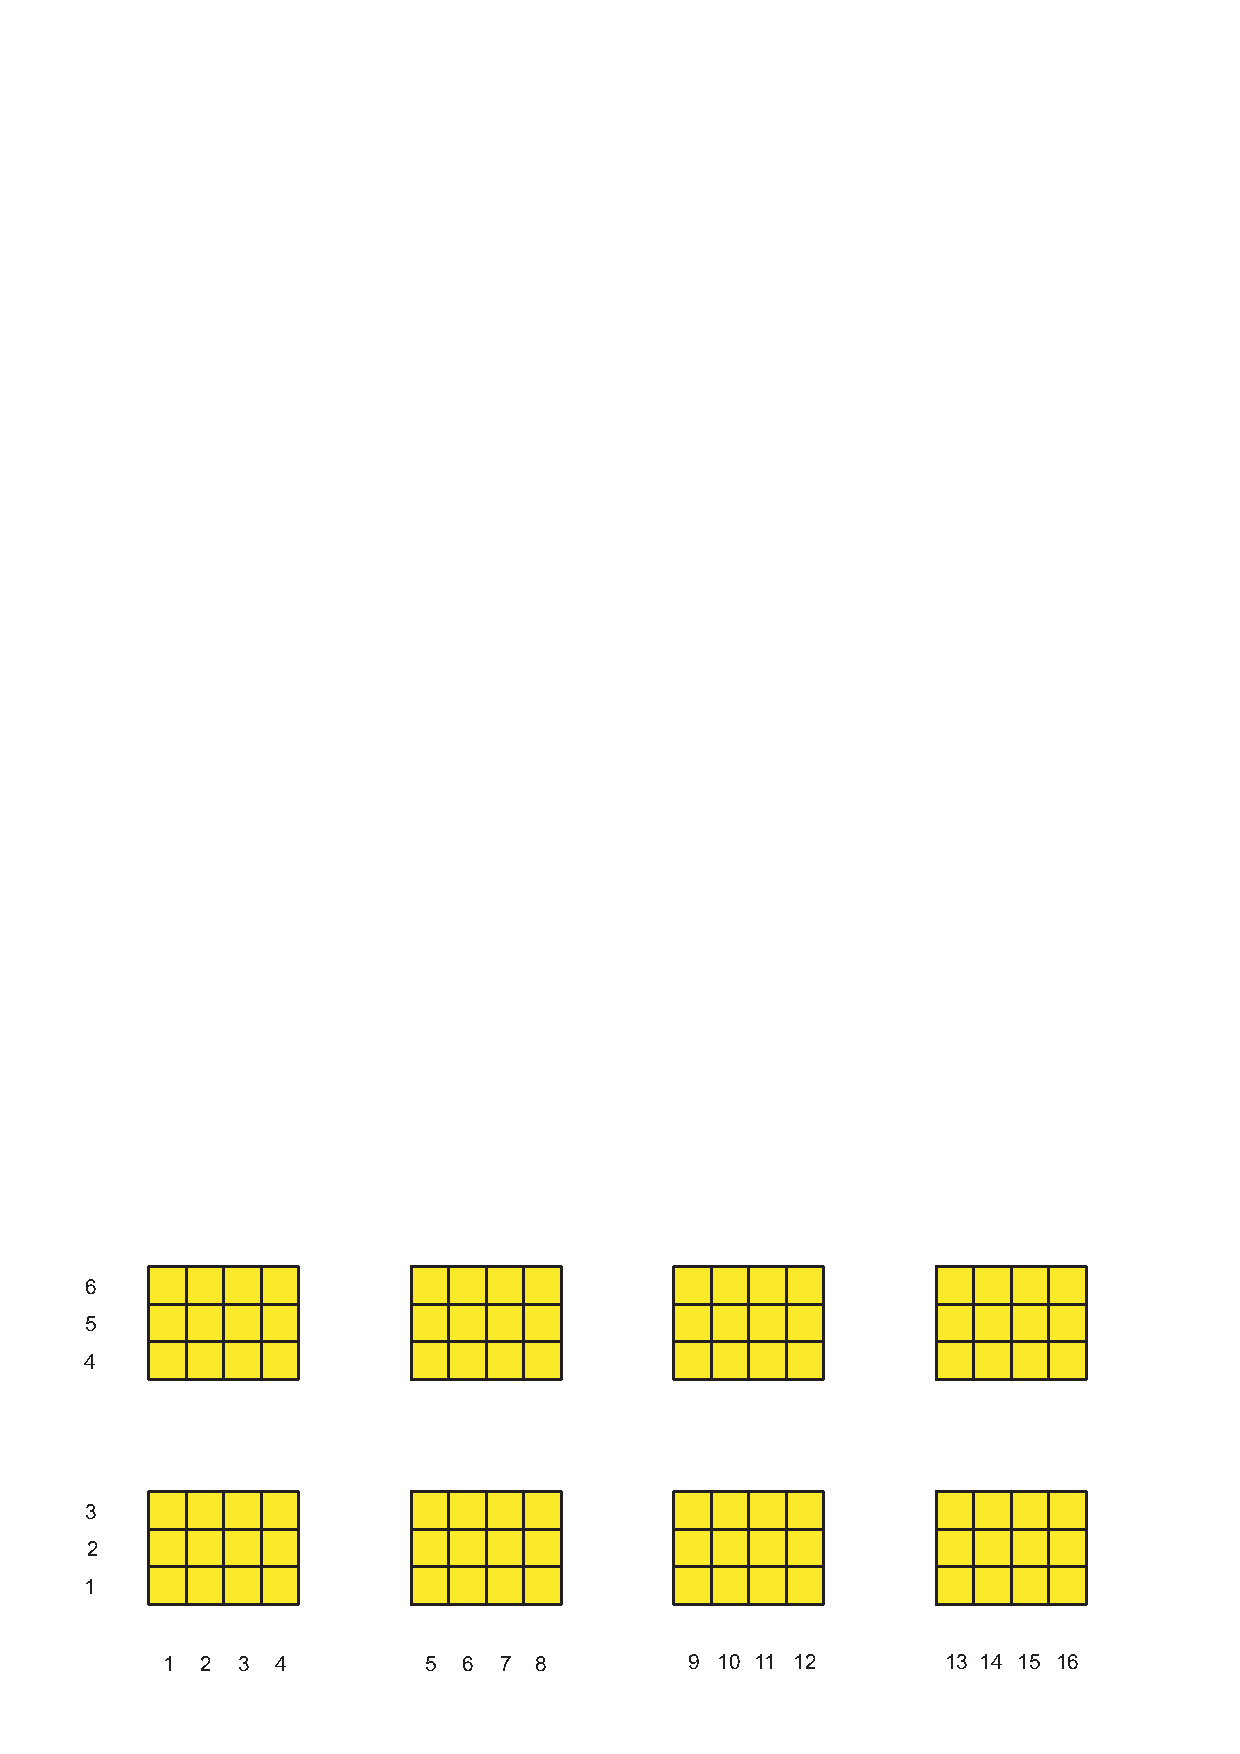
\includegraphics{GridExclusiveReg}}
  \caption{An example of a Grid's exclusive region for the corner stagger}
  \label{fig:gridexreg}
  \end{figure}
  \end{center}
  
   Figure~\ref{fig:gridexreg} shows an example of a Grid exclusive region for the
   {\tt ESMF\_STAGGERLOC\_CORNER} stagger with default
   stagger padding. This exclusive region would be for a Grid generated by either of the
   following calls: 
%/////////////////////////////////////////////////////////////

 \begin{verbatim}
  grid2D=ESMF_GridCreateNoPeriDim(regDecomp=(/2,4/), maxIndex=(/5,15/), &
           indexflag=ESMF_INDEX_GLOBAL, rc=rc)
 
\end{verbatim}
 
%/////////////////////////////////////////////////////////////

 \begin{verbatim}
  grid2D=ESMF_GridCreateNoPeriDim(countsPerDEDim1=(/4,4,4,3/), &
           countsPerDEDim2=(/3,2/), indexflag=ESMF_INDEX_GLOBAL, rc=rc)
 
\end{verbatim}
 
%/////////////////////////////////////////////////////////////

   Each rectangle in this diagram represents a DE and the numbers along the sides
   are the index values of the locations in the DE. Note that the exclusive region
   has one extra index location in each dimension than the number of cells
   because of the padding for the larger corner stagger location.
  
   The computational region is a user-settable region which can be used
   to distinguish a particular area for computation. The Grid doesn't
   currently contain functionality to let the user set the computational
   region so it defaults to the exclusive region. However, if the
   user sets an Array holding different computational bounds into the
   Grid then that Array's computational bounds will be used.
  
   The total region is the outermost boundary of the memory allocated
   on each DE to hold the data for the stagger location on that DE. This region
   can be as small as the exclusive region, but may be larger to
   include space for halos, memory padding, etc. The total region is
   what is enlarged to include space for halos, and the total region
   must be large enough to contain the maximum halo operation on the
   Grid. The Grid doesn't currently contain functionality to let the
   user set the total region so it defaults to the exclusive region.
   However, if the
   user sets an Array holding different total bounds into the
   Grid then that Array's total bounds will be used.
  
   The user can retrieve a set of bounds for each index space region
   described above: exclusive bounds, computational bounds,
   and total bounds. Note that although some of these are similar
   to bounds provided by ESMF\_Array subroutines
   (see Section~\ref{Array_regions_and_default_bounds})
   the format here is different. The Array bounds are only for
   distributed dimensions and are ordered to correspond
   to the dimension order in the associated DistGrid. The bounds
   provided by the Grid are ordered according to the order of dimensions of the data
   in question. This means that the bounds provided should be usable
   "as is" to access the data.
  
   Each of the three types of bounds refers to the maximum and minimum
   per dimension of the index ranges of a particular region. The parameters
   referring to the maximums contain a 'U' for upper. The parameters referring
   to the minimums contain an 'L' for lower. The bounds and associated
   quantities are almost always given on a per DE basis. The three types of
   bounds {\tt exclusiveBounds}, {\tt computationalBounds}, and {\tt totalBounds} refer
   to the ranges of the exclusive region, the computational region, and the
   total region. Each of these bounds also has a corresponding count parameter
   which gives the number of items across that region (on a DE) in each dimension.
   (e.g. {\tt totalCount(d)=totallUBound(i)-totalLBound(i)+1}). Width parameters
   give the spacing between two different types of region. The
   {\tt computationalWidth} argument gives the spacing between the exclusive
   region and the computational region. The {\tt totalWidth} argument gives the
   spacing between the total region and the computational region. Like the
   other bound information these are typically on a per DE basis, for example
   specifying {\tt totalLWidth=(1,1)} makes the bottom of the total
   region one lower in each dimension than the computational region on
   each DE. The exceptions to the per DE rule are
   {\tt staggerEdgeWidth}, and {\tt gridEdgeWidth}
   which give the spacing only on the DEs along the boundary of the Grid.
  
   All the above bound discussions only apply to the grid with non-arbitrary distributions,
   i.e., regular or irregular distributions.  For an arbitrarily distributed grid,
   only center stagger location is supported and there is no padding around the grid.
   Thus, the exclusive bounds, the total bounds and the computational bounds are identical
   and {\tt staggerEdgeWidth}, and {\tt gridEdgeWidth} are all zeros. 
%/////////////////////////////////////////////////////////////

  \subsubsection{Get Grid coordinate bounds}
  
   When operating on coordinates the user may often wish to
   retrieve the bounds of the piece of coordinate data on
   a particular local DE. This is useful for iterating through the
   data to set coordinates, retrieve coordinates, or do calculations.
   The method {\tt ESMF\_GridGetCoord} allows the user
   to retrieve bound information for a particular coordinate
   array.
  
   As described in the previous section there are three types of bounds the user can
   get: exclusive bounds, computational bounds,
   and total bounds. The bounds
   provided by {\tt ESMF\_GridGetCoordBounds} are for both distributed
   and undistributed dimensions and are ordered according to the
   order of dimensions in the  coordinate. This means that the bounds
    provided should be usable
   "as is" to access data in the coordinate array. In the case
   of factorized coordinate Arrays where a coordinate may
   have a smaller dimension than its associated Grid, then
   the dimension of the coordinate's bounds are the dimension of
   the coordinate, not the Grid.
  
   The following is an example of retrieving the bounds for localDE 0 for the first
   coordinate array from the corner stagger location. 
%/////////////////////////////////////////////////////////////

 \begin{verbatim}
   call ESMF_GridGetCoordBounds(grid2D, coordDim=1, localDE=0,  &
          staggerLoc=ESMF_STAGGERLOC_CORNER,                         &
          exclusiveLBound=elbnd, exclusiveUBound=eubnd,              &
          computationalLBound=clbnd, computationalUBound=cubnd,      &
          totalLBound=tlbnd, totalUBound=tubnd, rc=rc)
 
\end{verbatim}
 
%/////////////////////////////////////////////////////////////

  \subsubsection{Get Grid stagger location bounds}
  
   When operating on data stored at a particular stagger
   in a Grid the user may find it useful to be able
   to retrieve the bounds of the data on a particular local DE.
   This is useful for iterating through the
   data for computations or allocating arrays to hold the data.
   The method {\tt ESMF\_GridGet} allows the user
   to retrieve bound information for a particular stagger location.
  
   As described in Section~\ref{sec:grid:usage:bounds} there are three types of bounds
   the user can typically get, however, the Grid doesn't hold data at
   a stagger location (that is the job of the Field), and so
   no Array is contained there and so no total region exists, so the
   user may only retrieve exclusive and computational bounds from
   a stagger location.  The bounds
   provided by {\tt ESMF\_GridGet} are ordered according to the
   order of dimensions in the Grid.
  
   The following is an example of retrieving the bounds for localDE 0
   from the corner stagger location. 
%/////////////////////////////////////////////////////////////

 \begin{verbatim}
   call ESMF_GridGet(grid2D, localDE=0,                         &
          staggerLoc=ESMF_STAGGERLOC_CORNER,                    &
          exclusiveLBound=elbnd, exclusiveUBound=eubnd,         &
          computationalLBound=clbnd, computationalUBound=cubnd, rc=rc)
 
\end{verbatim}
 
%/////////////////////////////////////////////////////////////

  \subsubsection{Get Grid stagger location information}
  
   In addition to the per DE information that can be accessed about
   a stagger location there is some global information that can
   accessed by using {\tt ESMF\_GridGet} without specifying a
   localDE. One of the uses of this information is to create
   an ESMF Array to hold data for a stagger location.
  
   \begin{sloppypar}
   The information currently available from a stagger
   location is the {\tt distgrid}. The {\tt distgrid} gives the
   distgrid which describes the size and distribution of the elements in the stagger location.
   \end{sloppypar}
  
   The following is an example of retrieving information for localDE 0
   from the corner stagger location. 
%/////////////////////////////////////////////////////////////

 \begin{verbatim}
    ! Get info about staggerloc
    call ESMF_GridGet(grid2D, staggerLoc=ESMF_STAGGERLOC_CORNER,  &
           distgrid=staggerDistgrid, &
           rc=rc)

 
\end{verbatim}
 
%/////////////////////////////////////////////////////////////

  \subsubsection{Create an Array at a stagger location}
  
   In order to create an Array to correspond to a Grid stagger location
   several pieces of information need to be obtained from both the
   Grid and the stagger location in the Grid.
  
   The information that needs to be obtained from the Grid
   is the {\tt distgridToGridMap} to ensure that the new Array
   has its  dimensions are mapped correctly to the Grid. These
   are obtained using the {\tt ESMF\_GridGet} method.
  
   The information that needs to be obtained from the stagger
   location is the distgrid that describes the size and distribution
   of the elements in the stagger location. This information can
   be obtained using the stagger location specific {\tt ESMF\_GridGet} method.
  
   The following is an example of using information from a 2D Grid with non-arbitrary
   distribution to create an Array corresponding to a stagger location.
   
%/////////////////////////////////////////////////////////////

 \begin{verbatim}

    ! Get info from Grid
    call ESMF_GridGet(grid2D, distgridToGridMap=distgridToGridMap, rc=rc)
 
\end{verbatim}
 
%/////////////////////////////////////////////////////////////

 \begin{verbatim}

    ! Get info about staggerloc
    call ESMF_GridGet(grid2D, staggerLoc=ESMF_STAGGERLOC_CORNER, &
           distgrid=staggerDistgrid, &
           rc=rc)
 
\end{verbatim}
 
%/////////////////////////////////////////////////////////////

 \begin{verbatim}


    ! construct ArraySpec
    call ESMF_ArraySpecSet(arrayspec, rank=2, typekind=ESMF_TYPEKIND_R8, rc=rc)
 
\end{verbatim}
 
%/////////////////////////////////////////////////////////////

 \begin{verbatim}


    ! Create an Array based on info from grid
    array=ESMF_ArrayCreate(arrayspec=arrayspec, &
            distgrid=staggerDistgrid, distgridToArrayMap=distgridToGridMap, &
            rc=rc)

 
\end{verbatim}
 
%/////////////////////////////////////////////////////////////

   Creating an Array for a Grid with arbitrary distribution is different.
   For a 2D Grid with both dimension arbitrarily distributed, the Array dimension
   is 1.  For a 3D Grid with two arbitrarily distributed dimensions and one
   undistributed dimension, the Array dimension is 2.  In general,
   if the Array does not have any ungridded dimension, the Array dimension
   should be 1 plus the number of undistributed dimensions of the Grid.
  
   The following is an example of creating an Array for a 3D Grid with 2
   arbitrarily distributed dimensions such as the one defined in Section~\ref{example:ArbGridWithUndistDim}. 
%/////////////////////////////////////////////////////////////

 \begin{verbatim}
    ! Get distGrid from Grid
    call ESMF_GridGet(grid3D, distgrid=distgrid, rc=rc)
 
\end{verbatim}
 
%/////////////////////////////////////////////////////////////

 \begin{verbatim}


    ! construct ArraySpec
    call ESMF_ArraySpecSet(arrayspec, rank=2, typekind=ESMF_TYPEKIND_R8, rc=rc)
 
\end{verbatim}
 
%/////////////////////////////////////////////////////////////

 \begin{verbatim}


    ! Create an Array based on the presence of distributed dimensions
    array=ESMF_ArrayCreate(arrayspec=arrayspec,distgrid=distgrid, rc=rc)

 
\end{verbatim}
 
%/////////////////////////////////////////////////////////////

  \subsubsection{Create more complex Grids using DistGrid}
  \label{sec:usage:adv:create}
  
   Besides the shortcut methods for creating a Grid object such as
   {\tt ESMF\_GridCreateNoPeriDim()}, there is
   a set of methods which give the user more control over the
   specifics of the grid.  The following describes the more
   general interface, using DistGrid.
   The basic idea is to first create an ESMF DistGrid object describing
   the distribution and shape of the Grid, and then to employ that to either directly
   create the Grid or first create Arrays and then create the Grid from those.
   This method gives the user maximum control over the topology and distribution of the Grid.
   See the DistGrid documentation in Section~\ref{sec:DistGrid} for an
   in-depth description of its interface and use.
  
   As an example, the following call constructs
   a 10x20 Grid with a lower bound of (1,2). 
%/////////////////////////////////////////////////////////////

 \begin{verbatim}
   ! Create DistGrid
   distgrid2D = ESMF_DistGridCreate(minIndex=(/1,2/), maxIndex=(/11,22/), &
           rc=rc)
 
\end{verbatim}
 
%/////////////////////////////////////////////////////////////

 \begin{verbatim}

   ! Create Grid
   grid3D=ESMF_GridCreate(distGrid=distgrid2D, rc=rc)
 
\end{verbatim}
 
%/////////////////////////////////////////////////////////////

   \begin{sloppypar}
   To alter which dimensions are distributed, the {\tt distgridToGridMap}
   argument can be used. The {\tt distgridToGridMap} is used to set
   which dimensions of the Grid are mapped to the dimensions
   described by {\tt maxIndex}. In other words, it describes how the dimensions of
   the underlying default DistGrid are mapped to the Grid. Each entry
   in {\tt distgridToGridMap} contains the Grid dimension to which the corresponding
   DistGrid dimension should be mapped.
   The following example illustrates the creation of a Grid where the largest
   dimension is first. To accomplish this the two dimensions are swapped.
   \end{sloppypar} 
%/////////////////////////////////////////////////////////////

 \begin{verbatim}
   ! Create DistGrid
   distgrid2D = ESMF_DistGridCreate(minIndex=(/1,2/), maxIndex=(/11,22/), &
        rc=rc)
 
\end{verbatim}
 
%/////////////////////////////////////////////////////////////

 \begin{verbatim}

   ! Create Grid
   grid2D=ESMF_GridCreate(distGrid=distgrid2D, distgridToGridMap=(/2,1/), &
        rc=rc)
 
\end{verbatim}
 
%/////////////////////////////////////////////////////////////

  \subsubsection{Specify custom stagger locations}
  \label{sec:usage:staggerloc:adv}
  
   Although ESMF provides a set of predefined stagger locations (See Section~\ref{const:staggerloc}),
   the user may need one outside this set. This section describes the construction of
   custom stagger locations.
  
   To completely specify a stagger for an arbitrary number of dimensions, we define the
   stagger location in terms of a set of cartesian coordinates. The cell is represented
   by a n-dimensional cube with sides of length 2, and the coordinate origin located at
   the center of the cell. The geometry of the cell is for reference purposes only,
   and does not literally represent the actual shape of the cell. Think of this method
   instead as an easy way to specify a part (e.g. center, corner, face) of a higher
   dimensional cell which is extensible to any number of dimensions.
  
   To illustrate this approach, consider a 2D cell. In 2 dimensions
   the cell is represented by a square. An xy axis is placed at its center, with the
   positive x-axis oriented {\em East} and the positive y-axis oriented {\em North}.
   The resulting coordinate for the lower left corner is at $(-1,-1)$, and upper right
   corner at $(1,1)$.
   However, because our staggers are symmetric they don't need to distinguish between
   the $-1$, and the $1$, so we only need to concern ourselves with the first quadrant of
   this cell. We only need to use the $1$, and the $0$, and many of the cell locations
   collapse together (e.g. we only need to represent one corner). See figure~\ref{fig:gridcuststaggerloc}
   for an illustration of these concepts.
  
  \begin{center}
  \begin{figure}
  \center
  \scalebox{0.75}{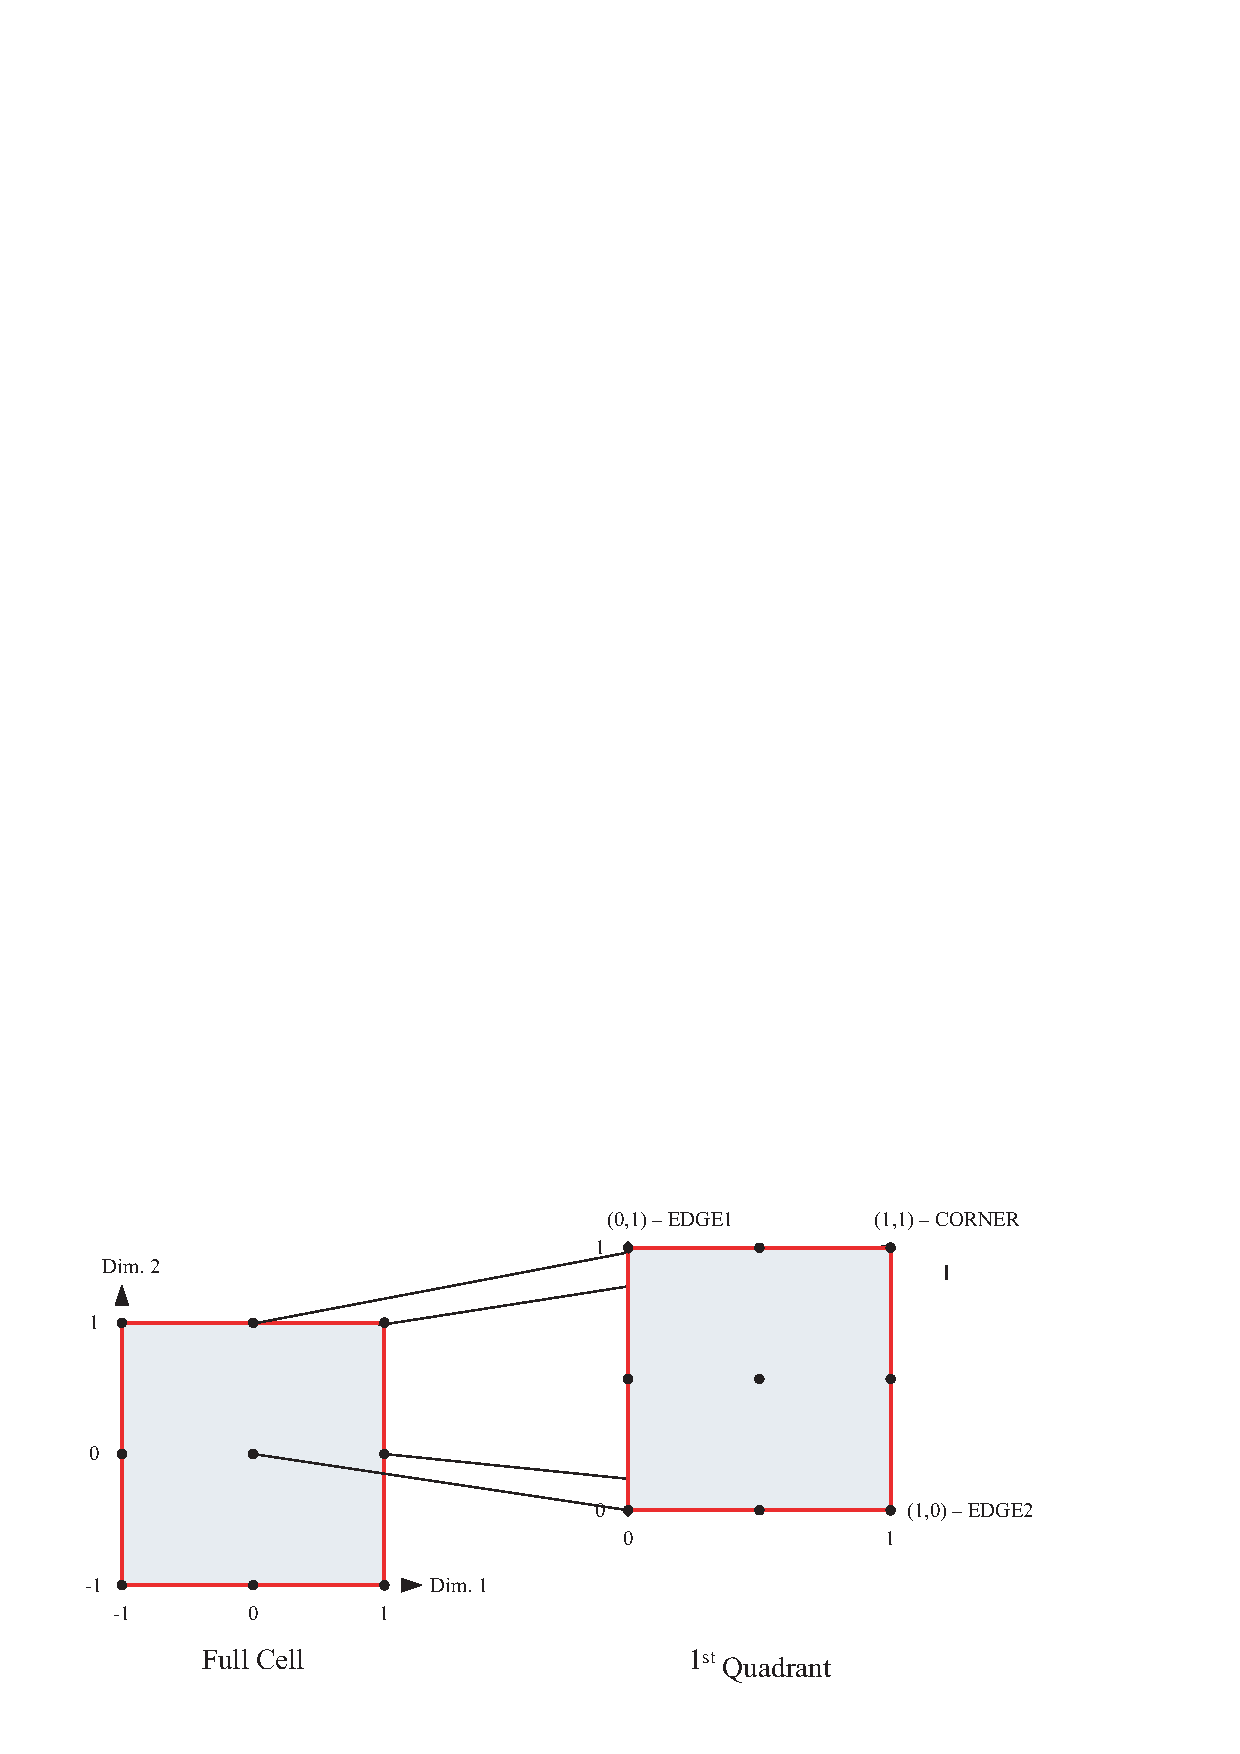
\includegraphics{GridCustStaggerLoc}}
  \caption{An example of specifying 2D stagger locations using coordinates.}
  \label{fig:gridcuststaggerloc}
  \end{figure}
  \end{center}
  
   The cell center is represented by the coordinate pair $(0,0)$ indicating the origin.
   The cell corner is $+1$ in each direction, giving a coordinate pair of $(1,1)$.
   The edges are each $+1$ in one dimension and $0$ in the other indicating that
   they're even with the center in one dimension and offset in the other.
  
   For three dimensions, the vertical component of the stagger location can be added by
   simply adding an additional coordinate. The three dimensional generalization of the
   cell center becomes $(0,0,0)$ and the cell corner becomes $(1,1,1)$. The rest of
   the 3D stagger locations are combinations of $+1$ offsets from the center.
  
   To generalize this to $d$ dimensions, to represent a $d$ dimensional stagger
   location. A set of $d$ $0$ and $1$ is used to specify for each dimension
   whether a stagger location is aligned with the cell center in that dimension ($0$),
   or offset by $+1$ in that dimension ($1$). Using this scheme we can represent
   any symmetric stagger location.
  
   To construct a custom stagger location in ESMF the subroutine
   {\tt ESMF\_StaggerLocSet()} is used to specify,
   for each dimension, whether the stagger is located at the interior (0)
   or on the boundary (1) of the cell. This method allows users
   to construct stagger locations for which
   there is no predefined value. In this example, it's used to
   set the 4D center and 4D corner locations.
   
%/////////////////////////////////////////////////////////////

 \begin{verbatim}

   ! Set Center
   call ESMF_StaggerLocSet(staggerLoc,loc=(/0,0,0,0/),rc=rc)
 
\end{verbatim}
 
%/////////////////////////////////////////////////////////////

 \begin{verbatim}
   call ESMF_GridAddCoord(grid4D, staggerLoc=staggerLoc, rc=rc)
 
\end{verbatim}
 
%/////////////////////////////////////////////////////////////

 \begin{verbatim}


   ! Set Corner
   call ESMF_StaggerLocSet(staggerLoc,loc=(/1,1,1,1/),rc=rc)
 
\end{verbatim}
 
%/////////////////////////////////////////////////////////////

 \begin{verbatim}

   call ESMF_GridAddCoord(grid4D, staggerLoc=staggerLoc, rc=rc)
 
\end{verbatim}
 
%/////////////////////////////////////////////////////////////

  \subsubsection{Specify custom stagger padding}
  \label{sec:usage:staggerpadding:adv}
  
  There is an added complication with the data (e.g. coordinates) stored at stagger locations in
  that they can require different amounts of storage depending
  on the underlying Grid type.
  
  \begin{center}
  \begin{figure}
  \center
  \scalebox{0.75}{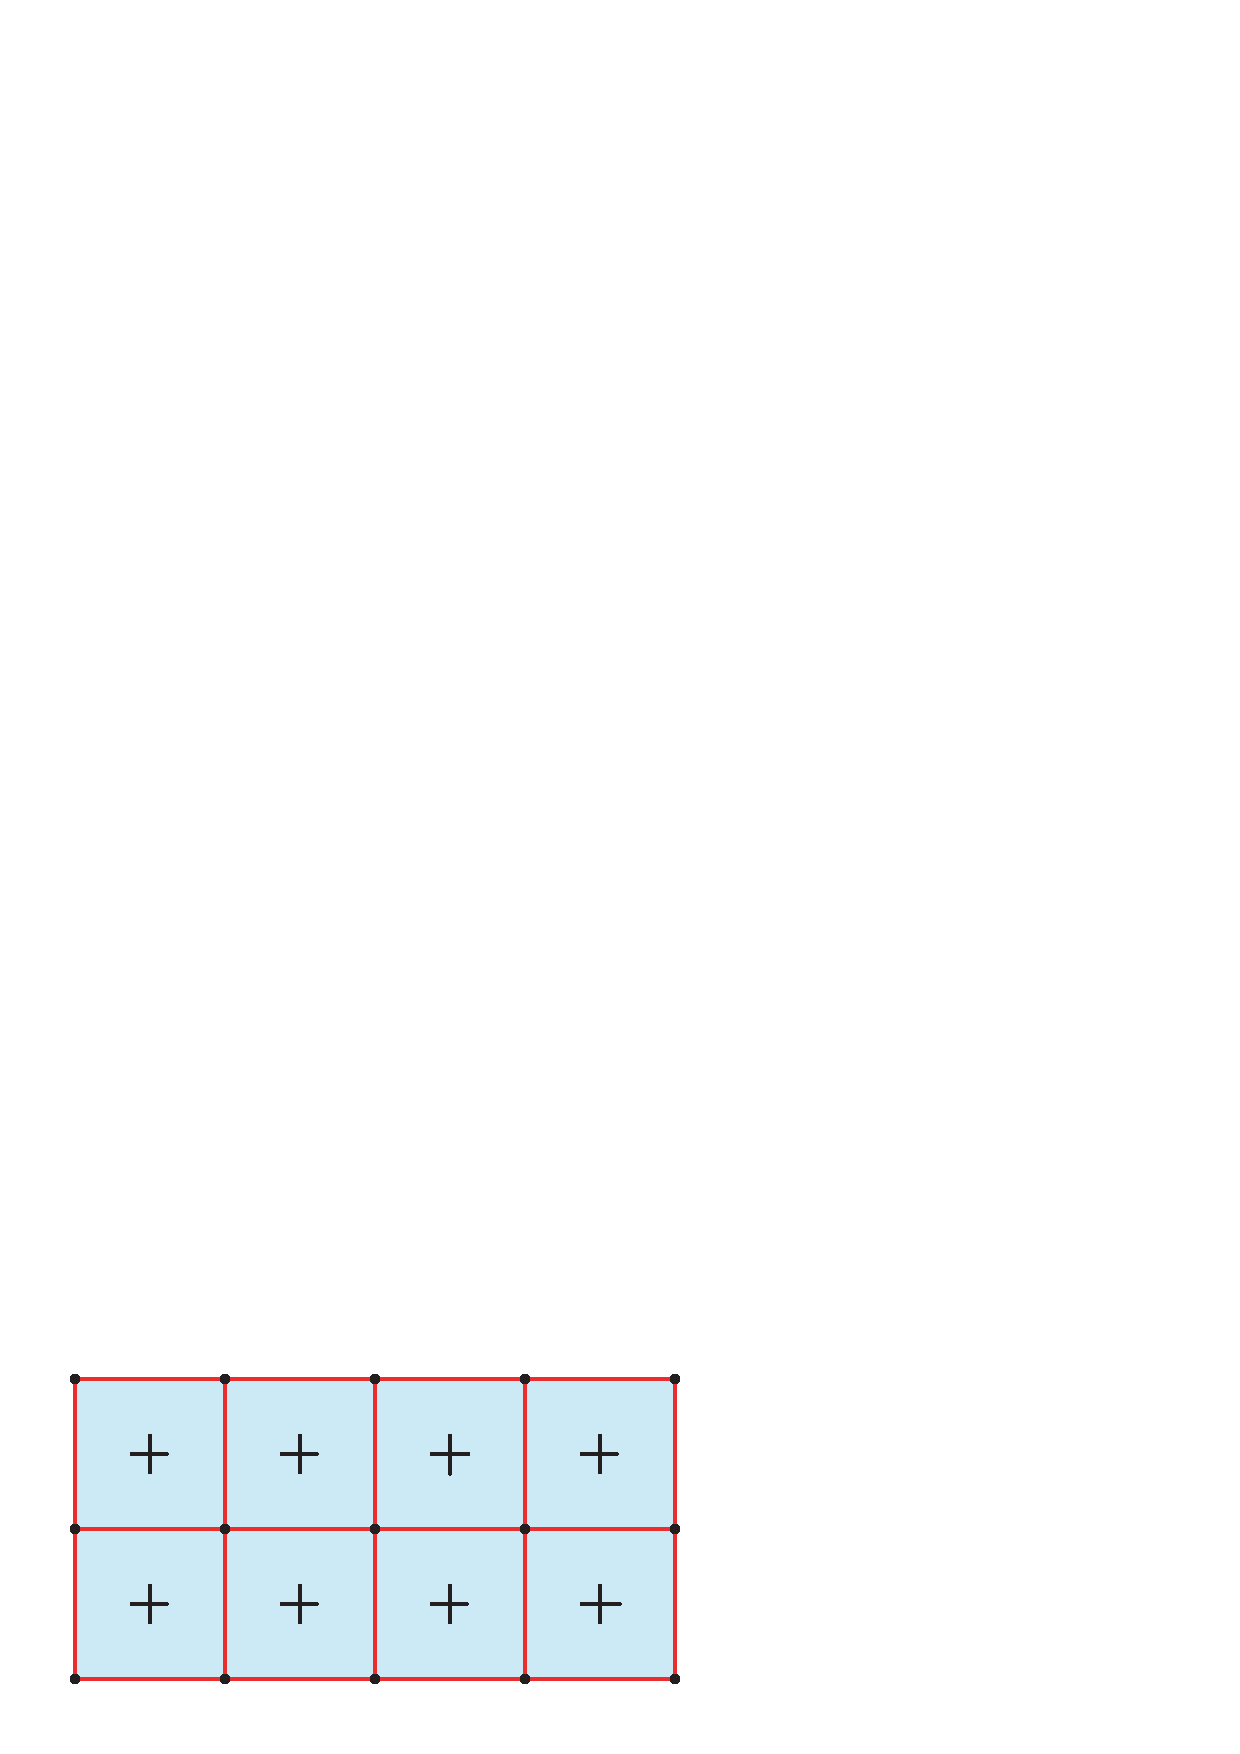
\includegraphics{GridCellsAndCorners}}
  \caption{An example 2D Grid with cell centers and corners.}
  \label{fig:gridcellsandcorners}
  \end{figure}
  \end{center}
  
   Consider the example 2D grid in figure~\ref{fig:gridcellsandcorners}, where the dots represent the cell corners
   and the ``+'' represents the cell centers. For the corners to completely
   enclose the cell centers (symmetric stagger), the number of corners in each
   dimension needs to be one greater then the number of cell centers. In the above
   figure, there are two rows and three columns of cell centers. To enclose the
   cell centers, there must be three rows and four columns of cell corners.
   This is true in general for Grids without periodicity or
   other connections.  In fact, for a symmetric stagger, given that the center
   location requires n x m storage, the corresponding corner location
   requires n+1 x m+1, and the edges, depending on the side, require n+1 x m or
   m+1 x n.  In order to add the extra storage, a new DistGrid is
   created at each stagger location. This Distgrid is similar to the DistGrid
   used to create the Grid, but has an extra set of elements added to hold the
   index locations for the stagger padding.
   By default, when the coordinate arrays are created, one extra
   layer of padding is added to the index space to create symmetric staggers
   (i.e. the center location is surrounded). The default is to add this padding
   on the positive side, and to only add this padding where needed
   (e.g. no padding for the center, padding
   on both dimensions for the corner, in only one dimension for the
   edge in 2D.) There are two ways for the user to change
   these defaults.
  
   One way is to use the {\tt GridEdgeWidth} or {\tt GridAlign} arguments
   when creating a Grid. These arguments can be used to change the default padding
   around the Grid cell index space. This extra padding is used by default
   when setting the padding for a stagger location.
  
   The {\tt gridEdgeLWidth} and
   {\tt gridEdgeUWidth} arguments are both 1D arrays of the
   same size as the Grid dimension. The entries in the arrays
   give the extra offset from the outer boundary of
   the grid cell index space. The following example shows the
   creation of a Grid with all the extra space to hold stagger padding
   on the negative side of a Grid. This is the reverse of
   the default behavior. The resulting Grid will have
   an exclusive region which extends from $(-1,-1)$ to
   $(10,10)$, however, the cell center stagger location
   will still extend from $(1,1)$ to $(10,10)$. 
%/////////////////////////////////////////////////////////////

 \begin{verbatim}
   grid2D=ESMF_GridCreateNoPeriDim(minIndex=(/1,1/),maxIndex=(/10,10/), &
            gridEdgeLWidth=(/1,1/), gridEdgeUWidth=(/0,0/), rc=rc)

 
\end{verbatim}
 
%/////////////////////////////////////////////////////////////

   To indicate how the data in a Grid's stagger locations are aligned with the
   cell centers, the optional {\tt gridAlign} parameter
   may be used. This parameter indicates which stagger elements
   in a cell share the same index values as the cell center.
   For example, in a 2D cell, it would indicate which of the four corners has
   the same index value as the center. To set {\tt gridAlign},
   the values -1,+1 are used to indicate the alignment in
   each dimension. This parameter is mostly
   informational, however, if the {\tt gridEdgeWidth} parameters
   are not set then its value determines where the default padding
   is placed. If not specified, then the default is to align all
   staggers to the most negative, so the padding is on the positive side.
   The following code illustrates creating a Grid aligned to the reverse of
   default (with everything to the positive side). This creates a
   Grid identical to that created in the previous example. 
%/////////////////////////////////////////////////////////////

 \begin{verbatim}
   grid2D=ESMF_GridCreateNoPeriDim(minIndex=(/1,1/),maxIndex=(/10,10/), &
            gridAlign=(/1,1/), rc=rc)

 
\end{verbatim}
 
%/////////////////////////////////////////////////////////////

   The {\tt gridEdgeWidth} and {\tt gridAlign} arguments both
   allow the user to set the default padding to be used
   by stagger locations in a Grid. By default, stagger locations
   allocated in a Grid set their stagger padding based on these
   values.  A stagger location's padding in each dimension is
   equal to the value of {\tt gridEdgeWidth} (or the value implied
   by {\tt gridAlign}), unless the stagger location is centered
   in a dimension in which case the stagger padding is 0. For example,
   the cell center stagger location has 0 stagger padding in all
   dimensions, whereas the edge stagger location lower padding
   is equal to {\tt gridEdgeLWidth} and the upper padding is equal
   to {\tt gridEdgeUWidth} in one dimension, but both are 0 in the other,
   centered, dimension.  If the user wishes to set the stagger padding
   individually for each stagger location they may use the
   {\tt staggerEdgeWidth} and {\tt staggerAlign} arguments.
  
   The {\tt staggerEdgeLWidth} and
   {\tt staggerEdgeUWidth} arguments are both 1D arrays of the
   same size as the Grid dimension. The entries in the arrays
   give the extra offset from the Grid cell index space
   for a stagger location. The following example shows the
   addition of two stagger locations. The
   corner location has no extra boundary and the
   center has a single layer of extra padding on
   the negative side and none on the positive.  This is the reverse of
   the default behavior. 
%/////////////////////////////////////////////////////////////

 \begin{verbatim}
   grid2D=ESMF_GridCreate(distgrid=distgrid2D, &
            gridEdgeLWidth=(/1,1/), gridEdgeUWidth=(/0,0/), rc=rc)
 
\end{verbatim}
 
%/////////////////////////////////////////////////////////////

 \begin{verbatim}


   call ESMF_GridAddCoord(grid2D, &
          staggerLoc=ESMF_STAGGERLOC_CORNER, &
          staggerEdgeLWidth=(/0,0/), staggerEdgeUWidth=(/0,0/), rc=rc)
 
\end{verbatim}
 
%/////////////////////////////////////////////////////////////

 \begin{verbatim}


   call ESMF_GridAddCoord(grid2D, &
          staggerLoc=ESMF_STAGGERLOC_CENTER, &
          staggerEdgeLWidth=(/1,1/), staggerEdgeUWidth=(/0,0/), rc=rc)

 
\end{verbatim}
 
%/////////////////////////////////////////////////////////////

   To indicate how the data at a particular stagger location is aligned with the
   cell center, the optional {\tt staggerAlign} parameter
   may be used. This parameter indicates which stagger elements
   in a cell share the same index values as the cell center.
   For example, in a 2D cell, it would indicate which of the four corners has
   the same index value as the center. To set {\tt staggerAlign},
   the values -1,+1 are used to indicate the alignment in
   each dimension. If a stagger location is
   centered in a dimension (e.g. an edge in 2D), then that
   dimension is ignored in the alignment. This parameter is mostly
   informational, however, if the {\tt staggerEdgeWidth} parameters
   are not set then its value determines where the default padding
   is placed. If not specified, then the default is to align all
   staggers to the most negative, so the padding is on the positive side.
   The following code illustrates aligning the positive (northeast in 2D)
   corner with the center. 
%/////////////////////////////////////////////////////////////

 \begin{verbatim}
   call ESMF_GridAddCoord(grid2D, &
          staggerLoc=ESMF_STAGGERLOC_CORNER, staggerAlign=(/1,1/), rc=rc)
 
\end{verbatim}

%...............................................................
\setlength{\parskip}{\oldparskip}
\setlength{\parindent}{\oldparindent}
\setlength{\baselineskip}{\oldbaselineskip}
